\chapter{AccessibleHub: Transforming mobile accessibility guidelines into code}
\label{chap:accessibility-toolkit}

\chapterintroline{
    This chapter introduces an accessibility learning toolkit for mobile developers. Building upon prior research, it provides a practical guide to implementing accessible mobile applications, particularly in Flutter. \textit{AccessibleHub}, a \gls{reactnative} toolkit, offers interactive examples and component-level guidance, comparing React Native and \gls{flutter}. Grounded in \gls{wcagg} principles, AccessibleHub aims to bridge the gap between accessibility guidelines and real-world application.
}

\section{Introduction}
\label{sec:intro}

\subsection{Challenges in implementing accessibility guidelines}

The importance of mobile app accessibility extends beyond mere compliance with legal regulations. Ensuring equal access to digital content and services is not only an ethical obligation but also a smart business decision. By prioritizing accessibility, app developers and companies can tap into a larger user base, improve user satisfaction, and demonstrate their commitment to social responsibility.
Despite the clear benefits and moral imperatives of mobile app accessibility, many developers still struggle to effectively implement accessibility guidelines in their projects. The \acrshort{wcagacr}, developed by the \gls{w3cg}, serve as the international standard for digital accessibility. However, translating these guidelines into practical implementation can be a challenging task, particularly starting from pure formal guidelines into everyday code. \\

One of the primary challenges lies in the complexity of the guidelines themselves. WCAG encompasses a wide range of \textit{success criteria}, organized under four main general \textit{principles}: perceivable, operable, understandable, and robust. Each principle contains multiple guidelines, and each guideline has several success criteria at different levels of \textit{conformance} (A, AA, AAA). Navigating this intricate web of requirements and understanding how to apply them to specific mobile app components can be overwhelming for developers, especially those new to accessibility. 
Moreover, the practical implementation of accessibility guidelines often varies across different platforms and frameworks. \textit{iOS} and \textit{Android}, the two dominant mobile operating systems, have their own unique accessibility \textit{API}s, tools, and best practices. Cross-platform frameworks like React Native and Flutter add another layer of complexity, as developers must ensure that their accessibility implementations are compatible with the underlying platform-specific mechanisms. \\ 

Furthermore, there is often a lack of clear, practical examples and guidance on how to implement accessibility features in real-world mobile app projects. While the \textit{WCAG} provides a solid foundation, it is primarily focused on web content and may not always directly address the unique challenges and interaction patterns of mobile apps. Developers often struggle to bridge the gap between the theoretical guidelines and the specific implementation details required for their projects.

\subsection{The need for practical developer education}

To address these challenges and bridge the gap between accessibility guidelines and practical implementation, there is a pressing need for developer education resources that focus on real-world, hands-on learning experiences. Traditional documentation and guidelines, while valuable, often fall short in providing the level of detail and interactivity needed to effectively guide developers through the accessibility implementation process.
This is where the concept of an \textit{accessibility learning toolkit} comes into play. An accessibility toolkit is designed to serve as a comprehensive, interactive resource that empowers developers to create accessible mobile applications by providing:

\begin{enumerate}
    \item Clear explanations of \acrshort{wcagacr} guidelines and their applicability to mobile apps;
    
    \item Step-by-step implementation guidance for common mobile app components and interaction patterns;
    
    \item Practical code examples and tutorials that demonstrate best practices;
    
    \item Hands-on exercises and challenges to reinforce learning and build confidence;
    
    \item Tools and techniques for testing and validating the accessibility of mobile apps.
\end{enumerate}

The primary goal of an accessibility learning toolkit is to bridge the gap between the theoretical knowledge of accessibility guidelines and the practical skills needed to implement them effectively in real-world projects. 
The toolkit should cater to developers at various levels of expertise, from beginners who are new to accessibility concepts to experienced professionals seeking to deepen their knowledge and stay up-to-date with the latest best practices. By providing a comprehensive, hands-on learning resource, the accessibility toolkit can play a crucial role in promoting a culture of inclusive design and development within the mobile app industry. \\

Current research, including Budai's work on Flutter accessibility testing, has primarily focused on end-user validation and testing methodologies. However, developers need practical, implementation-focused guidance that bridges multiple frameworks and platforms.
Despite widespread accessibility guidelines and standard, mobile application developers face significant challenges in translating theoretical requirements into practical implementations. This gap between guidelines and implementation is particularly evident in mobile development, where different platforms, screen sizes, and interaction models add complexity to accessibility implementation. Some of the most common challenges include:

\begin{itemize}
    \item Complex testing requirements - developers must validate across multiple devices, \gls{screenreaderg}, and interaction modes;
    
    \item Framework-specific implementations - each platform has unique accessibility \gls{apig}s and requirements;
    
    \item Limited practical examples - most documentation focuses on theoretical guidelines rather than concrete implementation patterns;
    
    \item Performance considerations - accessibility features must be implemented without compromising app performance.
\end{itemize}

Effective developer education in accessibility requires a solid grounding in learning theories that emphasize hands-on, interactive approaches. By integrating established learning theories with technical education principles, it's possible to justify the interactive and practical approach adopted in this toolkit. In doing so, we draw on constructivist and experiential learning models, which have been widely recognized as effective frameworks in technical and developer education.

Constructivist learning theories, pioneered by Piaget \cite{piaget1970science} and Vygotsky \cite{vygotsky1978mind}, posit that learning is an active process in which individuals construct knowledge based on their prior experiences and interactions with the environment. In the context of developer education, this suggests that hands-on learning is more effective than passive instruction \cite{savery2006overview}. By engaging with real-world accessibility challenges and actively experimenting with code implementations, developers can build a deeper understanding of accessibility guidelines and best practices, by having a tool at their disposal easy to use and to navigate. \\

Kolb's \textit{Experiential Learning Theory} \cite{kolb1984experiential} further supports this approach by describing learning as a four-stage cycle: concrete experience, reflective observation, abstract conceptualization, and active experimentation. For developers learning about accessibility, this cycle might involve encountering accessibility issues in their projects, analyzing existing solutions and guidelines, synthesizing their understanding of \acrshort{wcagacr} principles, and applying these principles to their own code. \textit{AccessibleHub} facilitates this learning cycle by providing a structured, interactive environment for developers to engage with accessibility concepts and implementations being organized into different core sections. By aligning with these proven pedagogical approaches, \textit{AccessibleHub} aims to provide an effective and engaging learning experience for developers. Moreover, by fostering a community of practice around accessibility while providing easier access to learning resources, this project encourages ongoing learning and knowledge sharing among developers, promoting the continuous improvement and dissemination of accessibility best practices.

\subsection{Research objectives and methodology}

Building upon previous research into mobile accessibility, this work aims to provide a comprehensive understanding of accessibility implementation across major cross-platform frameworks. While existing research indeed set grounds for both guidelines on accessibility and testing methodologies, there is a critical need to understand how these guidelines translate into practice for developers. 

This research addresses three fundamental questions about accessibility implementation in mobile development frameworks (referring to these ones as \textit{research questions}, following the work in \cite{perinello2024accessibility}:

\begin{itemize}
    \item First, we investigate whether components and widgets provided by frameworks are \textit{accessible by default}, without requiring additional developer intervention. This analysis is crucial for understanding the baseline accessibility support provided by each framework and identifying areas where additional implementation effort may be required;
    
    \item Second, we examine the \textit{feasibility of making non-accessible components accessible} through additional development effort. This involves analyzing the technical capabilities of each framework and identifying the necessary modifications to achieve accessibility compliance;
    
    \item Third, we quantify the \textit{development overhead required to implement accessibility features} when they are not provided by default. This includes measuring additional code requirements, analyzing complexity increases, and evaluating the impact on development workflows.
\end{itemize}

These questions is addressed via the usage of a systematic methodology aiming to address in detail accessibility support in React Native and Flutter, focusing on component implementation patterns and native platform integration. The implementation is comparative, allowing developers to directly implement accessible code examples with different degrees of implementation complexity measured quantitatively (including lines of code, required properties, and additional components needed for accessibility support). Comprehensive testing of implementations is also done using screen readers and other assistive technologies to verify accessibility compliance.

The \textit{goal} is to create an accessible application that serves three key purposes:
\begin{enumerate}
    \item To provide developers with practical, interactive examples of accessibility implementation, able to be copied easily and ported inside of other projects;
    
    \item To compare and contrast accessibility approaches between the main cross-development mobile frameworks in the current mobile landscape;
    
    \item To establish a reusable pattern library that demonstrates engine architecture, widget systems, and native platform integration, while ensuring compliance with current accessibility guidelines and legal requirements.
\end{enumerate}

The following sections will detail the development of \textit{AccessibleHub}, an application developed in React Native designed to serve as a practical manual for implementing accessibility features. While the technical aspects of cross-platform frameworks will be discussed later, the focus remains on providing developers with actionable implementation patterns and comparative insights for building accessible applications.

\section{React Native Overview}
\label{sec:reactnative-overview}

\gls{reactnative} is an open-source framework developed by Meta that enables developers to build mobile applications using JavaScript and the React paradigm (\cite{site:reactnative}). It employs a declarative, component-based approach through the use of \textit{JSX}, which is an XML-like syntax that allows developers to intermix JavaScript logic with markup. This combination not only improves code readability but also enhances modularity and facilitates code reuse.

\begin{figure}[ht]
    \centering
    
\includegraphics[width=0.4\textwidth, alt={React Native Logo}]{img/react-native-logo.png}
    \caption{React Native Logo}
\label{fig:reactnative-logo}
\end{figure}

\subsection{Core architecture and features}
\begin{itemize}
    \item \textit{Component-based architecture:}  
    The entire user interface in React Native is built from reusable components. Each component encapsulates its own logic and presentation, which greatly aids in the maintainability and scalability of complex applications;
    
    \item \textit{JSX syntax:}  
    Developers write the \acrshort{ui} using \textit{JSX}, a syntax extension similar to \textit{HTML}. This blending of code and layout simplifies the development process and enables a more intuitive understanding of the component structure;
    
    \item \textit{Bridging mechanism:}  
    React Native’s bridge enables asynchronous communication between the JavaScript layer and native modules. This means that while the application is written in JavaScript, performance-critical tasks can be executed using native code (e.g., Objective-C, Swift, or Java), ensuring a native look and feel without sacrificing performance;
    
    \item \textit{Hot reloading:}  
    One of the standout features present in this framework, which allows developers to see changes in real time without restarting the entire application. This accelerates the development cycle and aids in rapid prototyping;
    
    \item \textit{Unified codebase:}  
    React Native enables the development of applications for both iOS and Android using a single codebase. This unified approach reduces development time and effort compared to maintaining separate codebases for each platform.
\end{itemize}

\subsection{Accessibility in React Native}
React Native provides a robust set of accessibility features that are deeply integrated into its component model. This allows developers to create inclusive applications without relying on external libraries or writing platform-specific code (following what's present into \cite{site:reactnativeaccess}). Here are the key accessibility features in React Native:

\begin{itemize}
    \item \textbf{Accessibility properties}: React Native components can be enhanced with a variety of accessibility properties that provide semantic meaning and context for assistive technologies. These properties include:
    \begin{itemize}
        \item \texttt{accessibilityLabel}: A concise, descriptive string that identifies the component for screen reader users;
        \item \texttt{accessibilityRole}: Defines the component's semantic role (e.g., \texttt{"button"}, \texttt{"header"}), helping assistive technologies interpret its purpose correctly;
        \item \texttt{accessibilityHint}: Provides additional context about a component's function or the result of interacting with it;
        \item \texttt{accessibilityState}: Describes the current state of a component (e.g., \texttt{selected}, \texttt{disabled}), which is essential for conveying dynamic changes.
    \end{itemize}
    
    \item \textbf{Accessibility actions}: React Native allows developers to define custom accessibility actions for components, enabling advanced interactions beyond the default gestures. For example, a custom \texttt{accessibilityAction} could be added to a component to trigger a specific behavior when activated by an assistive technology;
    
    \item \textbf{Accessibility focus}: React Native manages accessibility focus automatically, ensuring that the correct component receives focus when navigating with assistive technologies. Developers can also programmatically control focus using the \texttt{accessibilityElementsHidden} and \\\texttt{importantForAccessibility} properties;
    
    \item \textbf{Accessibility events}: React Native provides accessibility events that notify assistive technologies when important changes occur in the application. These events include:
    \begin{itemize}
        \item \texttt{onAccessibilityTap}: Called when a user double-taps a component while using an assistive technology;
        \item \texttt{onMagicTap}: Called when a user performs the "magic tap" gesture (a double-tap with two fingers) to activate a component;
        \item \texttt{onAccessibilityFocus}: Called when a component receives accessibility focus;
        \item \texttt{onAccessibilityBlur}: Called when a component loses accessibility focus.
    \end{itemize}
\end{itemize}

By leveraging these built-in accessibility features, developers can create React Native applications that are inclusive and accessible to users with diverse needs and abilities. The tight integration of accessibility into the core component model ensures that developers can create accessible apps without sacrificing performance or maintainability.

\subsection{Advantages and developer benefits}

Using React Native offers several benefits for developers, briefly listed here:
\begin{itemize}
    \item \textit{Rapid development:}  
    Thanks to hot reloading and a vast ecosystem of reusable components, developers can iterate quickly and efficiently;
    
    \item \textit{Cross-platform consistency:}  
    With a unified codebase for both iOS and Android, developers can ensure a consistent user experience without duplicating effort;
    
    \item \textit{Integrated accessibility:}  
    React Native’s direct integration of accessibility properties allows developers to implement accessible features without having to rely on external tools or write platform-specific code;
    
    \item \textit{Community and support:}  
    A large and active community means extensive documentation, a wealth of third-party libraries, and a robust support network for troubleshooting and enhancements;
    
    \item \textit{Seamless transition for web developers:}  
    Developers familiar with React for web applications will find the transition to React Native smooth, as the core concepts and \textit{JSX} syntax remain consistent.
\end{itemize}

\subsection{Differences from native iOS/Android and web development}
\begin{itemize}
    \item \textit{Native iOS/Android:}  
    In native development, accessibility is handled through platform-specific \gls{apig}: \gls{voiceover} on \textit{iOS} and \gls{talkback} on \textit{Android}, which require different tools and approaches. React Native provides a unified \textit{API}s, streamlining the implementation of accessibility features across both platforms.
    
    \item \textit{Web development:}  
    Whereas web accessibility is achieved by adding \gls{ariag} attributes to \textit{HTML}, React Native integrates accessibility directly within its component structure. This intrinsic approach treats accessibility as a core attribute of each component, rather than an external addition.
\end{itemize}

In summary, React Native offers a modern, efficient, and developer-friendly environment that not only simplifies cross-platform mobile development but also incorporates accessibility into its core design. This makes it an ideal choice for creating inclusive applications, and it forms the foundational platform upon which the \textit{AccessibleHub} toolkit is built.

\section{AccessibleHub: An Interactive Learning Toolkit}
\label{sec:accessiblehub}

\subsection{Core architecture and design principles}

\textit{AccessibleHub} is a React Native application designed to serve as an interactive manual for implementing accessibility features in mobile development. Unlike traditional documentation or testing frameworks, the application provides developers with hands-on examples and implementation patterns that can be directly applied to their projects.

The application is structured around four conceptual main sections:
\begin{enumerate}
    \item \textit{Component examples}: Interactive demonstrations of common \acrshort{ui} elements with proper accessibility implementations, including buttons, forms, media content, and navigation patterns. This allows developers to clearly see the implementation of an accessible component and easily copy the code to their convenience;
    
    \item \textit{Framework comparison}: A detailed analysis of accessibility implementation approaches between React Native and Flutter, highlighting differences in component structure, properties, and required code;
    
    \item \textit{Testing tools}: Built-in utilities for validating accessibility features, allowing developers to understand how screen readers and other assistive technologies interact with their implementations;
    
    \item \textit{Implementation guidelines}: Technical documentation that connects WCAG requirements to practical code examples, providing clear paths for meeting accessibility standards.
\end{enumerate}

Each component presented serves dual purposes: demonstrating proper accessibility implementation while providing reusable code patterns. The application emphasizes practical implementation over theoretical guidelines, showing developers not just what to implement effectively. By focusing on developer experience, \textit{AccessibleHub} bridges the gap between accessibility requirements and actual implementation, providing a resource that can be directly integrated into the development workflow. \\

The \textit{design} philosophy of \textit{AccessibleHub} is founded on principles that bridge theoretical accessibility guidelines with practical implementation needs. While analyzing the current landscape of mobile development frameworks and accessibility implementation presented in \ref{chap:accessibility-literature}, a clear pattern emerges: developers need more practical, implementation-focused guidance that directly addresses the complexity of building accessible applications. To address this need, \textit{AccessibleHub} adopts three fundamental architectural principles:

\begin{enumerate}
    \item The usage of a \textit{component-first architecture}, where each UI element exists as an independent, self-contained unit demonstrating both implementation patterns and accessibility features. In other words, each one of them is being constructed within an \textit{accessibility-first} experience which ensures that usage of screen readers and other assistive technologies is kept as a priority. This modular approach provides two advantages: it first allows developers to comprehend and apply accessibility features in isolation, hence reducing cognitive load and implementation complexity, and enables systematic testing and validation of accessibility features of every component. Also, this means accessibility patterns can be studied, implemented, and verified in isolation from added complexity brought in by interactions among those components;

    \item \textit{Progressive enhancement} as a core design methodology. Instead of presenting accessibility as big challenge from the start, components are structured in increasing levels of complexity. This starts with basic elements like buttons and text inputs where basic accessibility patterns can be established. As developers master these foundational components, the application introduces more complex patterns such as forms, navigation systems, and gesture-based interactions. This helps into guiding the development towards more complicated scenarios;

    \item Focus on \textit{framework-agnostic patterns}, not depending on a specific framework while providing concrete code implementations. Even though \textit{AccessibleHub} has been implemented in React Native, all the patterns and principles explained are designed to transcend into specific framework implementations. The approach wants to give importance to the compatibility and reusability in the framework on the mobile development side. It will compare the implementations, mainly between React Native and Flutter, to show how developers can port accessibility patterns across different frameworks and understand core accessibility concepts in an easy-to-implement manner within professional projects. 
    
\end{enumerate}

Through these principles, \textit{AccessibleHub} aims to transform accessibility from an afterthought into an \textit{accessibility-by-design}. The application serves not just as a reference implementation, but as an educational tool that guides developers through the process of building truly accessible applications. This approach recognizes that effective accessibility implementation requires both theoretical understanding and practical experience, providing developers with the tools they need to create more inclusive mobile applications.

\subsection{Educational framework design}

\textit{AccessibleHub}'s educational framework is designed to provide a structured, incremental learning experience that progressively builds accessibility knowledge and skills. The content is organized into different \textit{learning modules}, each focusing on a key aspect of mobile accessibility. This is structured incrementally, so to help a developer gather a general idea on what needs to be implemented following a practical roadmap of steps: this allows to focus on different aspects of mobile accessibility, selecting each time the most relevant ones.

The core of the application is divided into different main screens, following:

\begin{enumerate}
    \item \textbf{Home} - The entry point for the \textit{AccessibleHub} application (\ref{fig:homescreen}). It provides an overview of the main sections and guides users on where to start their accessibility learning journey. The Home screen is designed to be intuitive and user-friendly, with clear call-to-action towards the accessible components section, allowing a developer or a user navigate to the desired section from the Home screen, comprehensive of comparison between the main mobile frameworks, learn about best practices in mobile accessibility and access testing tools documentation. There is also present a compliance dashboard provides an overview of an app's accessibility compliance status, based on the \acrshort{wcagacr} and \acrshort{mcagacr} guidelines. Developers can use this information to prioritize their accessibility efforts and focus on the areas that need the most attention;

    \begin{figure}[ht]
    \centering
    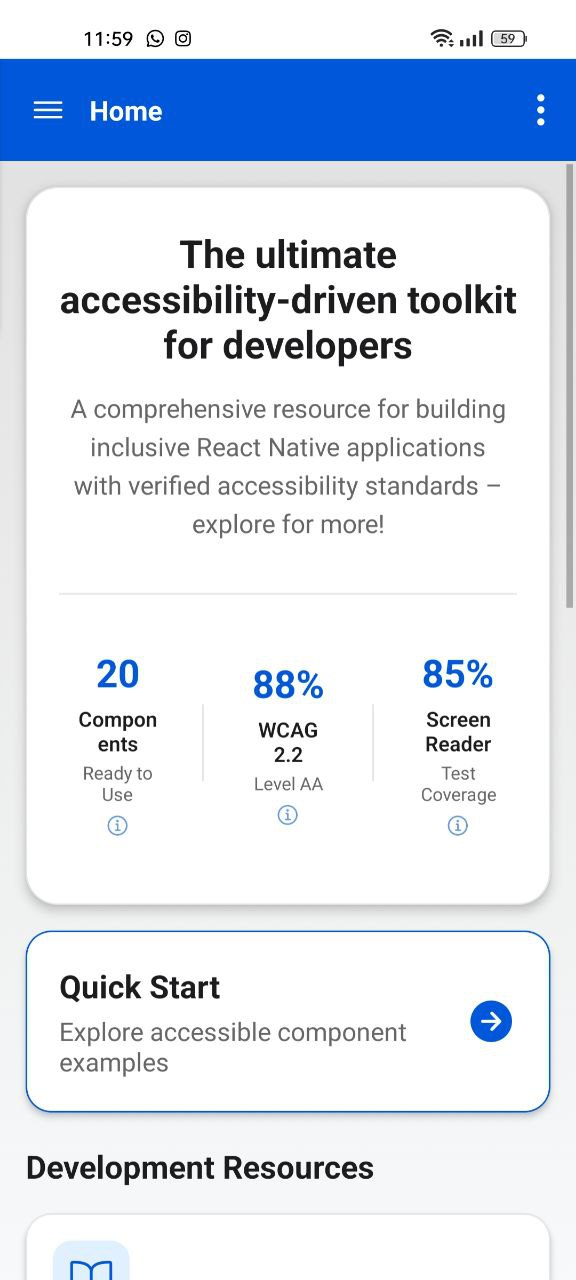
\includegraphics[width=0.4\linewidth, alt={Screenshot of the Home Screen of AccessibleHub}]{img/homescreen.jpg}
    \caption{The Home Screen of \textit{AccessibleHub}}\label{fig:homescreen}
    \end{figure}

\pagebreak

    \item \textbf{Accessible Components} - Developers can learn how to implement accessible UI components in their mobile applications (\ref{fig:components}). This section is divided into four subscreens, each focusing on a specific category of components:

    \begin{itemize}
        \item \textit{Buttons and Touchables}: It covers the implementation of accessible buttons and touchable elements. It provides code examples and best practices for ensuring that these interactive elements are perceivable, operable, and understandable by all users, including those with disabilities;

        \item \textit{Forms}: The subscreen focuses on creating accessible input forms, including text fields, checkboxes, radio buttons, and date/time pickers. It demonstrates how to properly label form elements, provide instructions and feedback, and ensure that forms can be navigated and completed using various input methods, such as keyboards and screen readers;

        \item \textit{Media}: In the Media subscreen, developers learn how to make media content, such as images, videos, and audio, accessible to users with visual or auditory impairments. This includes providing alternative text for images, captions for videos, and transcripts for audio content;

        \item \textit{Dialogs}: It covers the creation of accessible modal dialogs, popups, and alerts. It provides guidance on how to ensure that these elements are properly announced by screen readers, can be easily dismissed, and do not interfere with the user's ability to navigate the application, maintaining focus management and ensuring clear exit strategies;

       \item \textit{Advanced}: This particular subscreen covers elements like alerts, sliders, progress bars and tab navigation, analyzing how accessibility may regard different animated or interactive components for more complex gesture interactions used everyday by users.
    \end{itemize}

Throughout the Components section, code implementations are shared as examples, which developers can easily copy to their clipboard and integrate into their own projects. This hands-on approach allows developers to quickly apply the accessibility principles they learn and see the results in action.

\begin{figure}[ht]
\centering
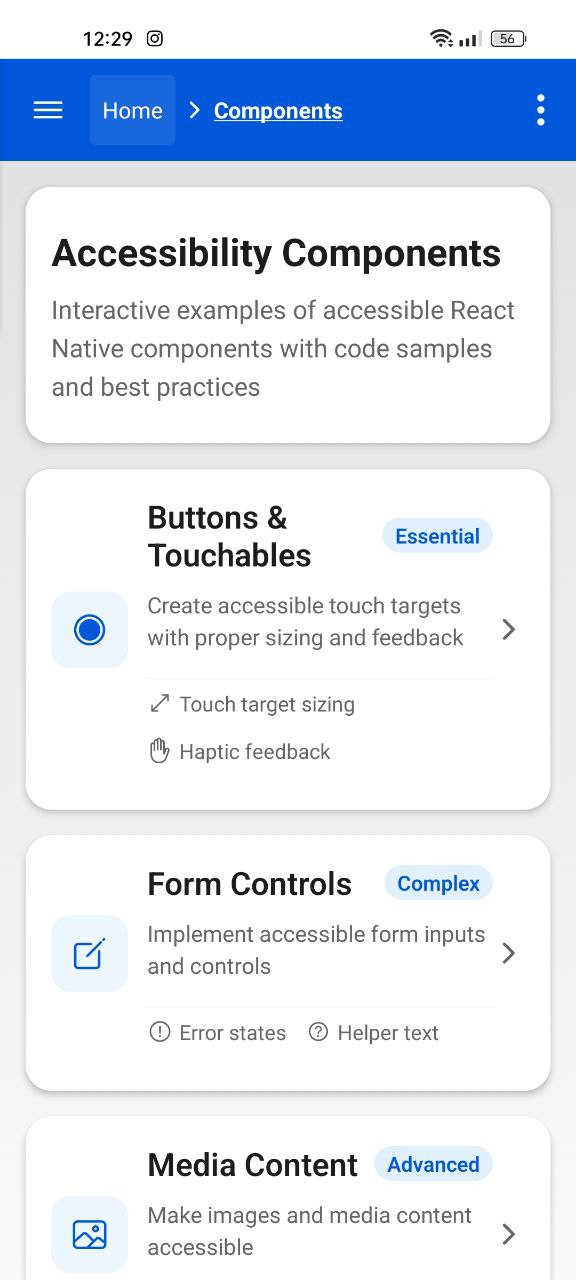
\includegraphics[width=0.4\linewidth, alt={Screenshot of the Components Screen of AccessibleHub}]{img/components.jpg}
\caption{The Components Screen of \textit{AccessibleHub}}\label{fig:components}
\end{figure}

\pagebreak

\item \textbf{Best Practices} - Designed to give developers a general understanding of the overarching principles and guidelines for creating accessible mobile applications (\ref{fig:best-practices}). It is divided into five subscreens, each addressing a key aspect of mobile accessibility:

    \begin{itemize}
        \item \textit{Gestures Tutorial}: This subscreen provides an overview of the various gesture interactions used in mobile applications and how to make them accessible to users with motor impairments or those relying on assistive technologies. It covers best practices for implementing alternative input methods and providing clear instructions and feedback. These gestures are general, tested to be used universally, both by everyday users and screen reader ones;

        \item \textit{Semantics Structure}: Here, developers learn about the importance of using semantic \textit{HTML} and \gls{ariag} roles to convey the structure and meaning of the application's content. This helps screen readers and other assistive technologies better understand and navigate the application;

        \item \textit{Navigation}: This one focuses on creating accessible navigation patterns, such as menus, tabs, and breadcrumbs. It provides guidance on how to ensure that navigation elements are properly labeled, can be operated using various input methods, and provide clear feedback to the user, jumping directly to the main context of a screen and bringing the attention to an element on-screen without distracting him from the action to be completed;

        \item \textit{Screen Reader Support}: This subscreen covers the specific considerations for making mobile applications compatible with screen readers, such as \gls{voiceover} on \textit{iOS} and \gls{talkback} on \textit{Android}. It includes best practices for labeling elements, providing alternative text, and ensuring that the application's content and functionality can be fully accessed and understood using a screen reader;

        \item \textit{Accessibility Guidelines}: The Accessibility Guidelines subscreen provides an overview of the key accessibility standards to be followed and a general list of principles to incorporate into a project, seeing how they apply to mobile application development. It helps developers understand the different levels of conformance and how to assess their application's accessibility against these guidelines.
    \end{itemize}

\begin{figure}[ht]
\centering
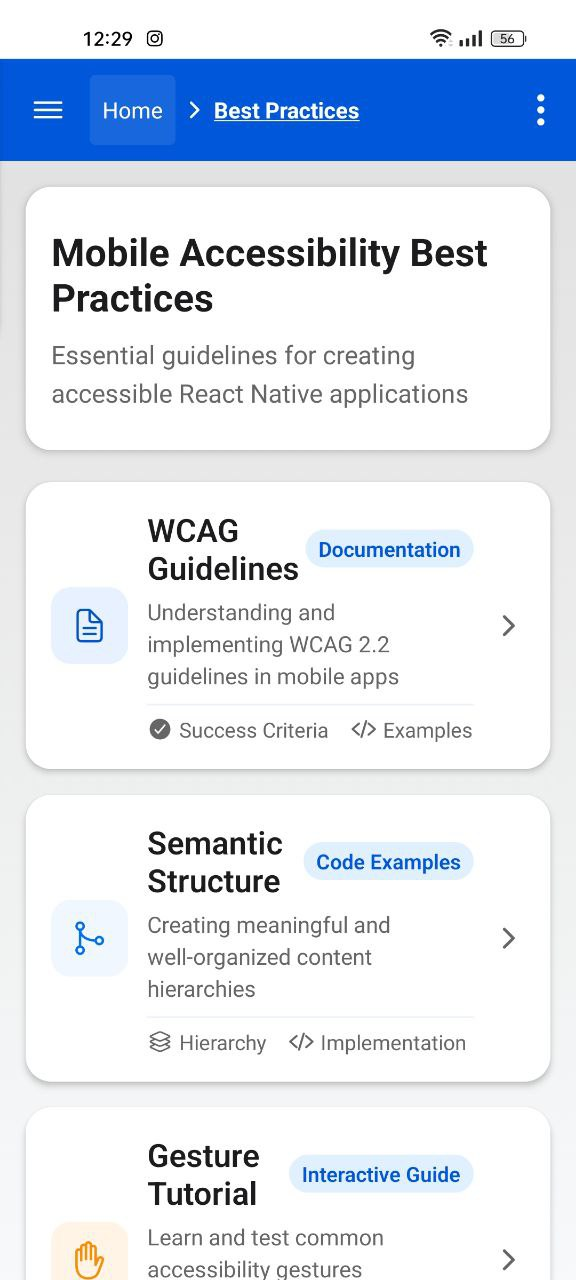
\includegraphics[width=0.4\linewidth, alt={Screenshot of the Best Practices Screen of AccessibleHub}]{img/best-practices.jpg}
\caption{The Best Practices Screen of \textit{AccessibleHub}}\label{fig:best-practices}
\end{figure}

\pagebreak

\item \textbf{Framework Comparison} - It provides a side-by-side comparison of the accessibility features and implementation differences between popular mobile development frameworks, such as React Native and Flutter (\ref{fig:frameworks-comparison}). This section helps developers understand how accessibility is handled in each framework and provides guidance on leveraging the specific accessibility APIs and tools available in each one. This is divided into different categories, offering a practical and formal overview on how such frameworks are compared with each other. By highlighting the similarities and differences between frameworks, developers can make informed decisions about which framework to use for their accessibility needs and how to optimize their implementations for each platform;

\begin{figure}[ht]
\centering
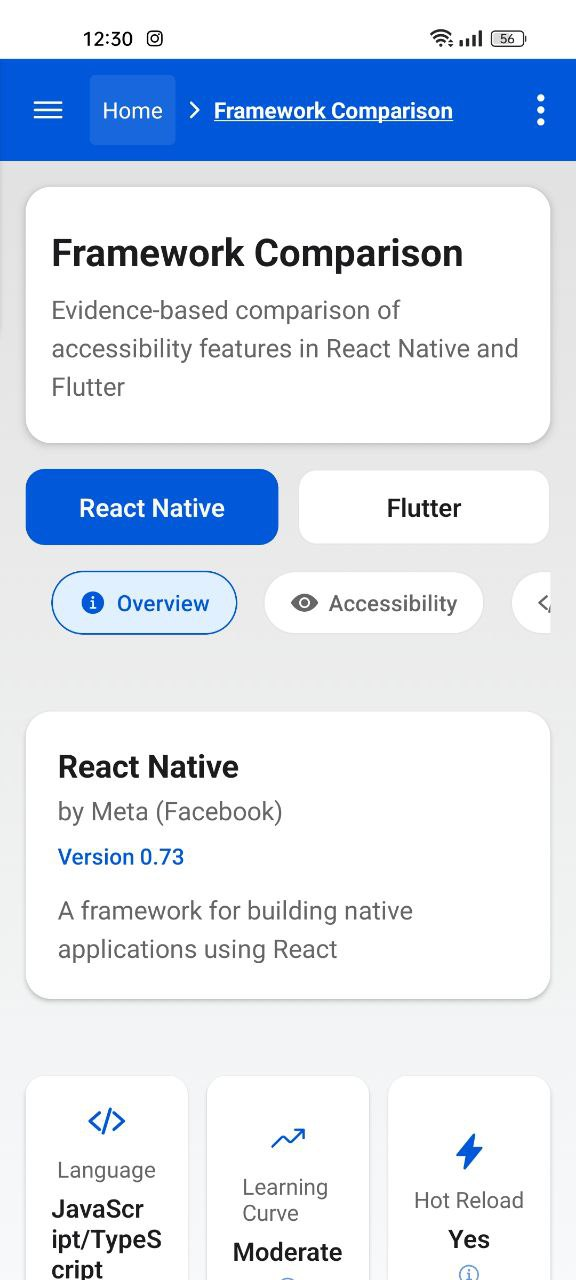
\includegraphics[width=0.4\linewidth, alt={Screenshot of the Frameworks Comparison Screen of AccessibleHub}]{img/frameworks-comparison.jpg}
\caption{The Frameworks Comparison Screen of \textit{AccessibleHub}}\label{fig:frameworks-comparison}
\end{figure}

\pagebreak

\item \textbf{Tools} - It serves as a central hub for accessing various accessibility-related tools and resources (\ref{fig:tools}). This includes links to official documentation, such as the React Native Accessibility \acrshort{api} reference and the \textit{Flutter Accessibility package} documentation. It also provides quick access to popular accessibility testing tools, such as \textit{Accessibility Scanner} for \textit{Android} and \textit{Accessibility Inspector} for \textit{iOS}. By consolidating these resources in one place, the Tools screen makes it easy for developers to find the information and tools they need to ensure their applications are fully accessible; 

\begin{figure}[ht]
\centering
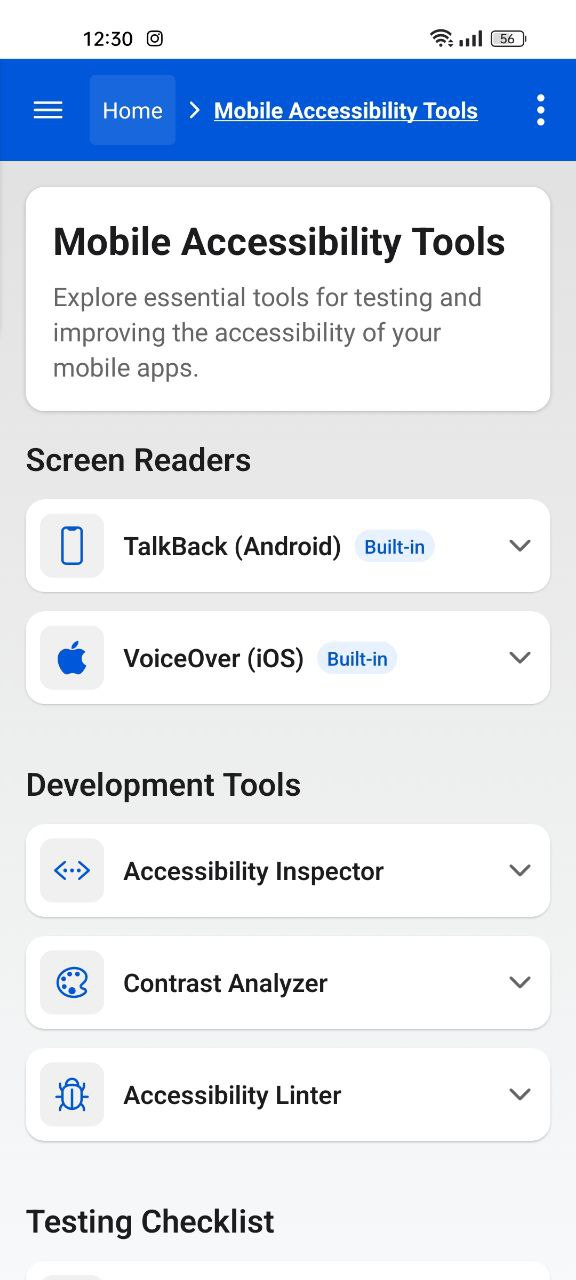
\includegraphics[width=0.4\linewidth, alt={Screenshot of the Tools Screen of AccessibleHub}]{img/tools.jpg}
\caption{The Tools Screen of \textit{AccessibleHub}}\label{fig:tools}
\end{figure}

\pagebreak

\item \textbf{Settings} - Allows users to customize various aspects of the \textit{AccessibleHub} application to suit their individual learning needs and preferences (\ref{fig:settings}). This includes options for adjusting the font size, color contrast (including options for gray scale and dark mode), reduced motion settings and others to help users and ensure the application itself is accessible to a wide range of users. It also provides information on how to configure the accessibility settings on the user's device, such as enabling screen readers or adjusting the display settings. By offering these customization options and guidance, the page reinforces the importance of accessibility as an everyday tool, meant to accompany practical user needs in an easy and quick way;

\begin{figure}[ht]
\centering
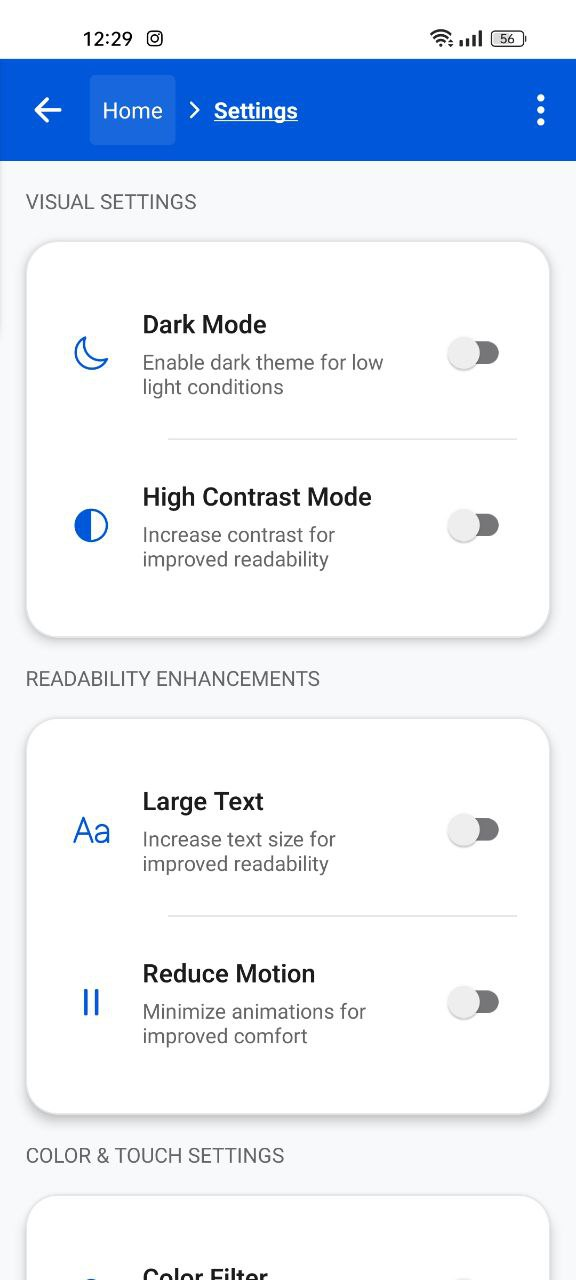
\includegraphics[width=0.4\linewidth, alt={Screenshot of the Settings Screen of AccessibleHub}]{img/settings.jpg}
\caption{The Settings Screen of \textit{AccessibleHub}}\label{fig:settings}
\end{figure}

\pagebreak

\item \textbf{Instruction and Community} - It provides a collaborative learning environment that extends beyond technical implementation (\ref{fig:instruction-community}). This section offers developers an opportunity to dive deeper into accessibility knowledge through curated resources and community engagement allowing for easier exploration towards other online resources. This provides an overview of currently open projects in the field of accessibility, provides advices on specific plugins and offers community examples of interest for a developers to be motivated into the creation of other accessible projects. By providing a platform for continuous learning and collaboration, this screen reinforces the importance of accessibility as a collective effort and a fundamental aspect of modern mobile application development.

\begin{figure}[ht]
\centering
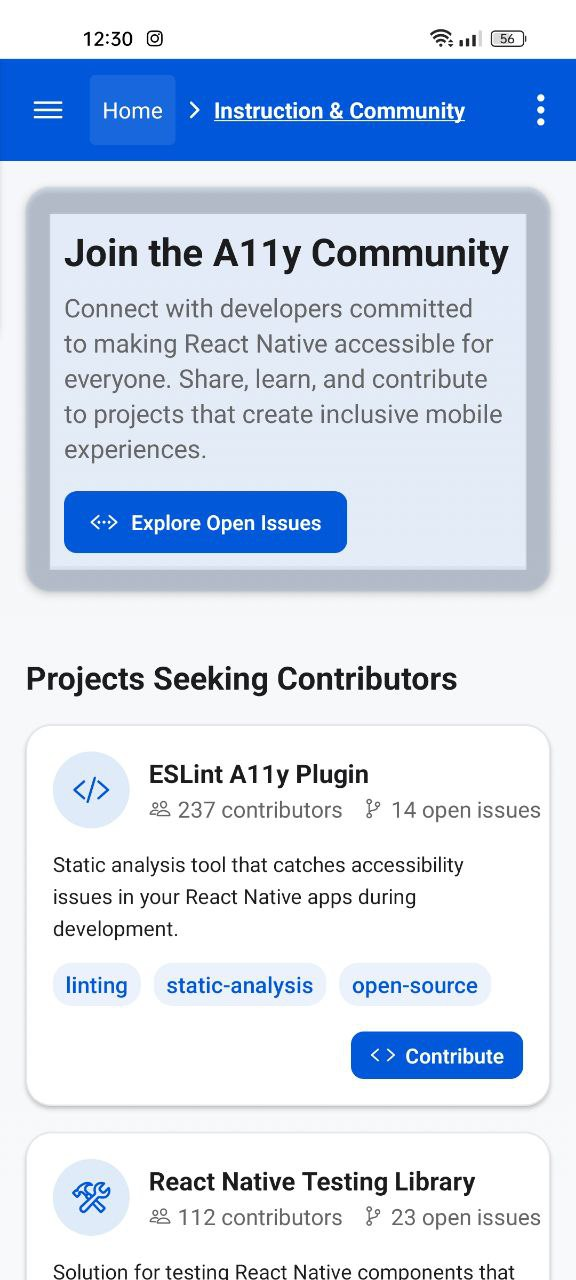
\includegraphics[width=0.4\linewidth, alt={Screenshot of the Instruction and Community Screen of AccessibleHub}]{img/instruction-community.jpg}
\caption{The Instruction and Community Screen of \textit{AccessibleHub}}\label{fig:instruction-community}
\end{figure}
    
\end{enumerate}

\pagebreak

\subsection{From guidelines to implementation: a screen-based methodology}

Accessibility guidelines and standards - most notably the \acrshort{wcagacr}  and related mobile-specific considerations—establish the formal foundation for inclusive digital design, as discussed in \ref{sec:accessibility-guidelines}. These criteria are essential but inherently abstract and can be challenging to implement directly in code. Building on Perinello and Gaggi's approach focusing solely on post-implementation testing, the methodology presented embeds accessibility into the development process. We do this by analyzing each screen of the application through a structured framework that connects theoretical requirements with practical implementation strategies. The approach to be considered is built following these layers:

\begin{enumerate}
    \item \textit{Theoretical foundation} – This layer encompasses the abstract principles and success criteria defined by \textit{WCAG}/\acrshort{mcagacr}. For example, \textit{WCAG}’s four core principles require that content be presented in ways users can perceive, interact with, and understand. These criteria serve as the benchmark for our analysis;

    \item \textit{Implementation pattern} – Here, we translate the abstract requirements into concrete code structures within a mobile development context. In \textit{AccessibleHub}, this involves the systematic use of React Native properties (such as \textit{accessibilityLabel}, \textit{accessibilityRole}, etc.) to ensure that \acrshort{ui} components satisfy the established guidelines;

    \item \textit{User interaction flow} – Finally, we consider how end users interact with these components. This includes the behavior of assistive technologies (like screen readers), proper focus management, and the overall usability of the component within its real-world context.
\end{enumerate}

To illustrate this methodology in practice, we first map the \textit{UI} elements of a representative screen to their corresponding semantic roles. Next, we link each component to the relevant \acrshort{wcagacr} and \acrshort{mcagacr} criteria presented in the previous subsections, noting both the minimum compliance requirements and potential enhancements. Finally, we describe the technical solution—specifically, how React Native accessibility code properties are applied to meet and exceed these standards. This structured approach not only bridges the gap between abstract guidelines and real-world coding tasks but also sets the stage for the more detailed, screen-by-screen analyses presented in the next section.

\section{Accessibility implementation guidelines}
\label{sec:implementation-guidelines}

Having established the overall architecture of \textit{AccessibleHub} and the guiding principles from both \textit{WCAG} and \textit{MCAG}, we now present a screen-by-screen analysis. Each subsection highlights the key \textit{success criteria} addressed, references relevant \textit{mobile-specific considerations}, and demonstrates practical solutions in React Native. Where applicable, we contrast these with Flutter's approach, building upon the insights from Gaggi and Perinello's approach \cite{budai2024mobile} analazying Budai's Flutter code - following guidelines and then giving advice into introducing new ones.

\subsection{Home screen}

The Home Screen serves as the primary entry point of the \textit{AccessibleHub} application. It provides key metrics on accessibility compliance (e.g., number of accessible components, \acrshort{wcagacr} conformance level) and direct navigation to core sections: \textit{Accessible Components} (Quick Start), \textit{Best Practices}, \textit{Testing Tools}, and the \textit{Framework Comparison}. An example of the interface is shown in Figure~\ref{fig:home_screens_sidebyside}.

\begin{figure}[ht]
    \centering
    \begin{subfigure}[b]{0.48\textwidth}
        \centering
        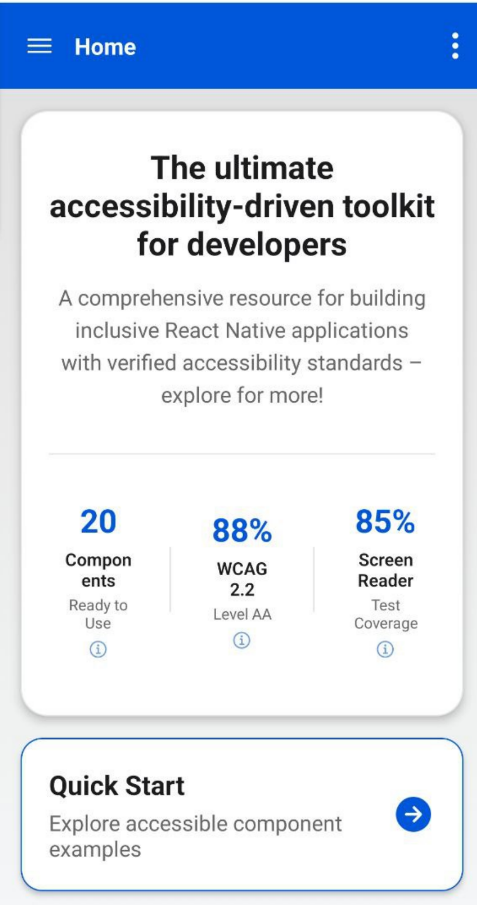
\includegraphics[width=\linewidth, alt={First part of the Home Screen}]{img/home1.png}
        \caption{Home screen - Part 1}
        \label{fig:home-left}
    \end{subfigure}
    \hfill
    \begin{subfigure}[b]{0.48\textwidth}
        \centering
        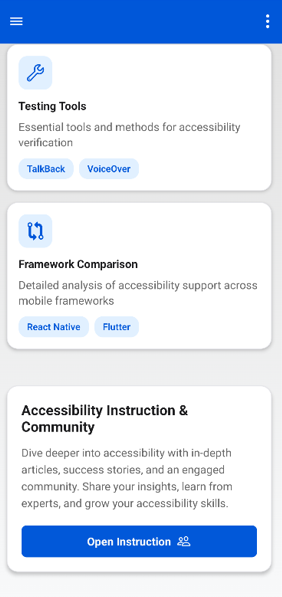
\includegraphics[width=\linewidth, alt={Second part of the Home Screen}]{img/home2.png}
        \caption{Home screen - Part 2}
        \label{fig:home-right}
    \end{subfigure}
    \caption{Side-by-side view of the two Home sections, with metrics and navigation buttons}
    \label{fig:home_screens_sidebyside}
\end{figure}

\subsubsection{Component inventory and WCAG/MCAG mapping}

Table~\ref{tab:component_criteria_mapping} provides a formal mapping between the UI components, their semantic roles, the specific WCAG 2.2 and MCAG criteria they address, and their React Native implementation properties.

\begin{longtable}{|p{2.5cm}|p{2cm}|p{2.8cm}|p{2.8cm}|p{4.3cm}|}
\caption{Home screen component-criteria mapping}
\label{tab:component_criteria_mapping}\\
\hline
\textbf{Component} & \textbf{Semantic Role} & \textbf{WCAG 2.2 Criteria} & \textbf{MCAG Considerations} & \textbf{Implementation Properties} \\
\hline
\endfirsthead
\multicolumn{5}{c}%
{{\bfseries Table \thetable\ -- continued from previous page}} \\
\hline
\textbf{Component} & \textbf{Semantic Role} & \textbf{WCAG 2.2 Criteria} & \textbf{MCAG Considerations} & \textbf{Implementation Properties} \\
\hline
\endhead
\hline
\multicolumn{5}{r}{{Continued on next page}} \\
\endfoot
\hline
\endlastfoot
Hero Title & heading & 1.4.3 Contrast (AA)\newline 2.4.6 Headings (AA) & Text readability on variable screen sizes & \texttt{accessibilityRole \ ="header"} \\
\hline
Stats Cards & button & 1.4.3 Contrast (AA)\newline 2.5.8 Target Size (AA)\newline 4.1.2 Name, Role, Value (A) & Touch target size\newline Non-essential information & \texttt{accessibilityRole \ ="button"}\newline \texttt{accessibilityLabel="\$\{value\}\% \$\{type\}, tap for details"}\newline \texttt{accessibilityHint="Shows \$\{type\} details"} \\
\hline
Decorative Icons & none & 1.1.1 Non-text Content (A) & Reduction of unnecessary focus stops & \texttt{accessibility \ ElementsHidden \ =true}\newline \texttt{important \ ForAccessibility="no"} \\
\hline
Quick Start Button & button & 1.4.3 Contrast (AA)\newline 2.5.8 Target Size (AA)\newline 2.5.2 Pointer Cancellation (A) & One-handed operation & \texttt{accessibilityRole \ ="button"}\newline \texttt{minHeight: 48}\newline \texttt{minWidth: 150} \\
\hline
Feature Cards & button & 1.3.1 Info and Relationships (A)\newline 1.4.3 Contrast (AA)\newline 2.5.8 Target Size (AA) & Logical grouping & \texttt{accessibilityRole \ ="button"}\newline \texttt{accessibilityLabel \ ="\$\{title\}"}\newline \texttt{accessibilityHint \ ="\$\{hint\}"} \\
\hline
Modal Dialog & dialog & 2.4.3 Focus Order (A)\newline 4.1.2 Name, Role, Value (A) & Keyboard trap prevention & \texttt{accessibilityRole \ ="dialog"}\newline Focus management implementation \\
\hline
Modal Tabs & tablist & 2.4.7 Focus Visible (AA)\newline 4.1.2 Name, Role, Value (A) & Touch interaction & \texttt{accessibilityRole \ ="tablist"}\newline \texttt{accessibility \ State= \ \{\{ selected: isActive \}\}} \\
\end{longtable}

\subsubsection{Formal metrics calculation methodology}

The Home Screen displays three key metrics that provide quantitative measurements of the application's accessibility. These metrics are not arbitrary but are calculated using a formal methodology defined in the \texttt{calculateAccessibilityScore} function within \texttt{index.tsx}. 

\begin{figure}[ht]
    \centering
    \begin{subfigure}[b]{0.48\textwidth}
        \centering
        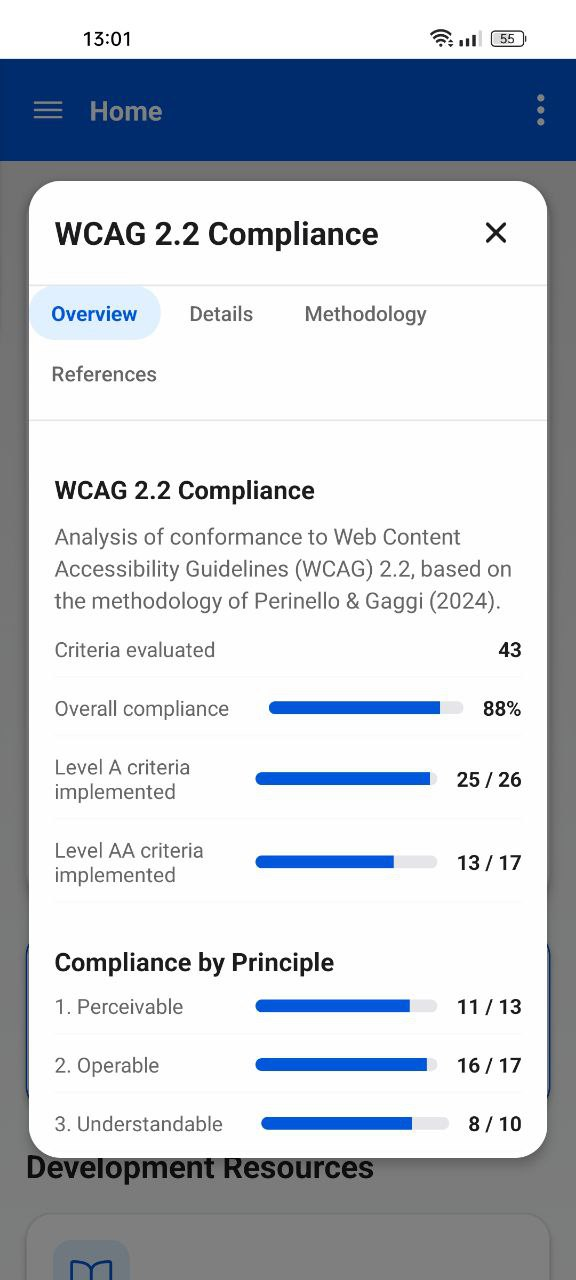
\includegraphics[width=\linewidth]{img/wcag-compliance.jpg}
        \caption{WCAG compliance overview}
        \label{fig:wcag-compliance-modal}
    \end{subfigure}
    \hfill
    \begin{subfigure}[b]{0.48\textwidth}
        \centering
        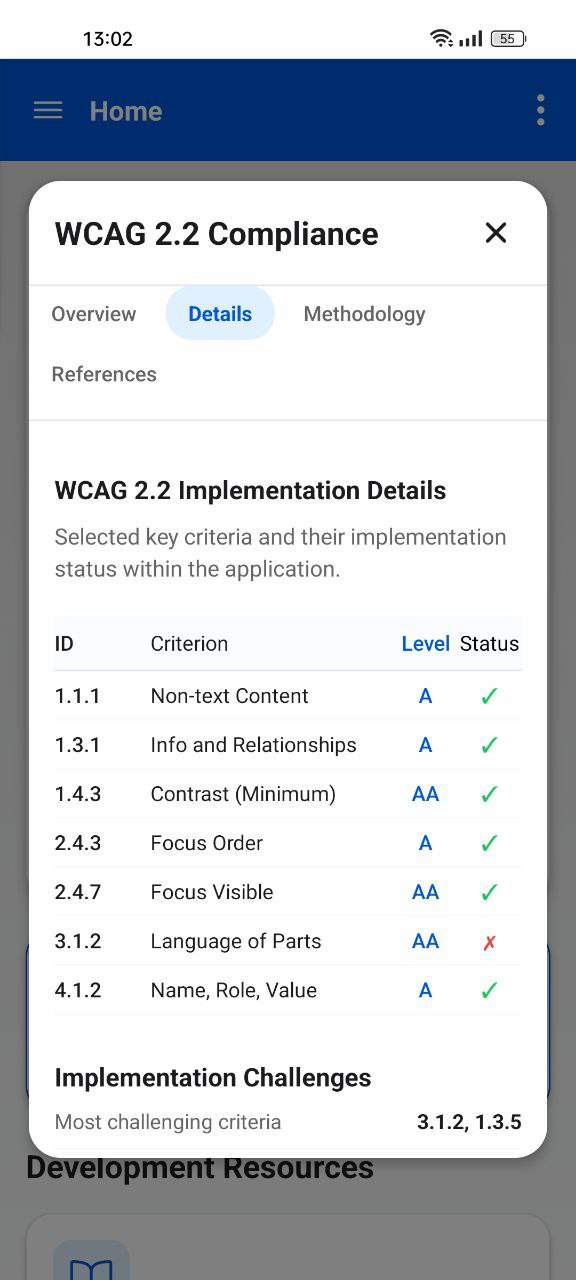
\includegraphics[width=\linewidth]{img/wcag-compliance-details.jpg}
        \caption{WCAG compliance details}
        \label{fig:wcag-details-modal}
    \end{subfigure}
    \caption{Modal dialogs showing WCAG compliance metrics}
    \label{fig:wcag_modal_pair}
\end{figure}

\begin{figure}[ht]
    \centering
    \begin{subfigure}[b]{0.48\textwidth}
        \centering
        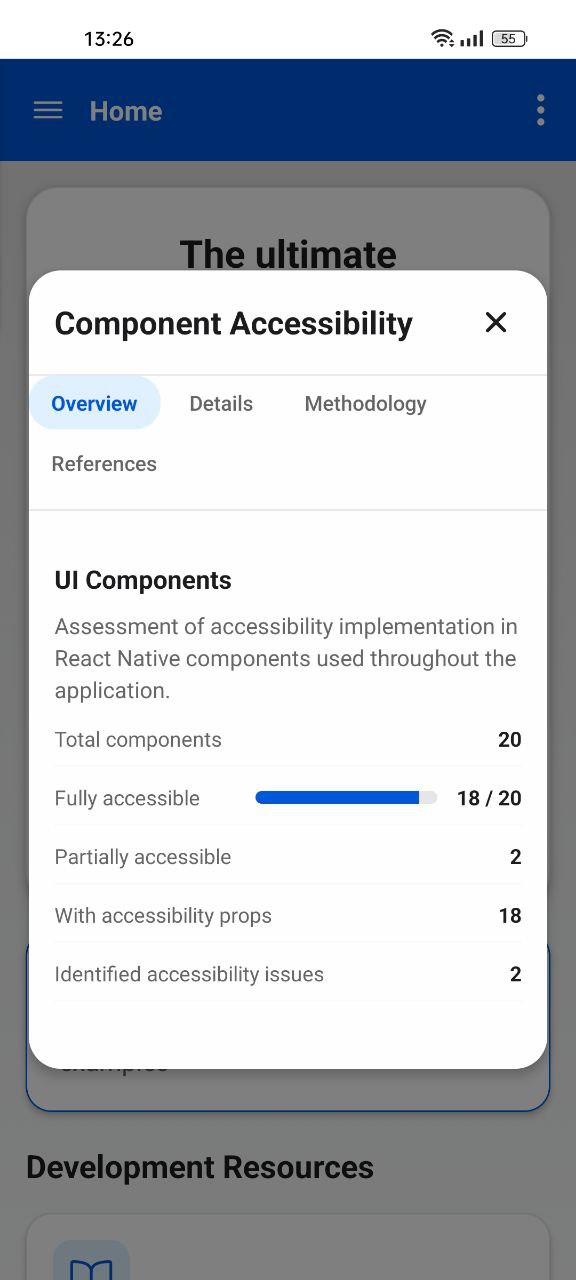
\includegraphics[width=\linewidth]{img/component-modal.jpg}
        \caption{Component metrics overview}
        \label{fig:component-overview-modal}
    \end{subfigure}
    \hfill
    \begin{subfigure}[b]{0.48\textwidth}
        \centering
        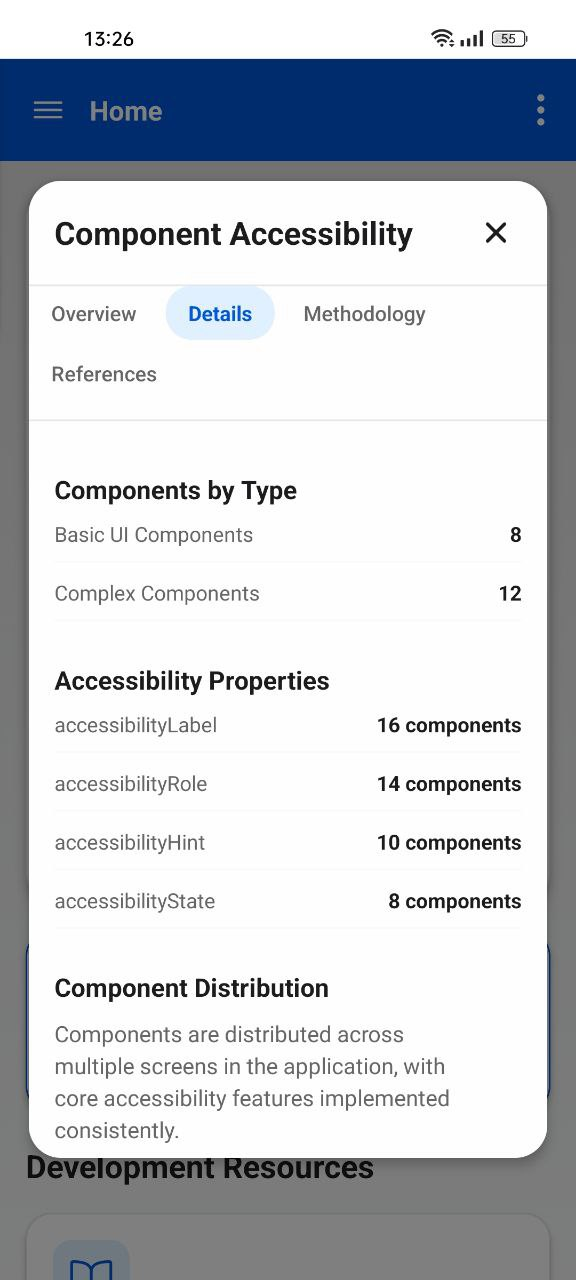
\includegraphics[width=\linewidth]{img/component-details.jpg}
        \caption{Component metrics details}
        \label{fig:component-details-modal}
    \end{subfigure}
    \caption{Modal dialogs showing component accessibility metrics}
    \label{fig:component_modal_pair}
\end{figure}

\begin{figure}[ht]
    \centering
    \begin{subfigure}[b]{0.48\textwidth}
        \centering
        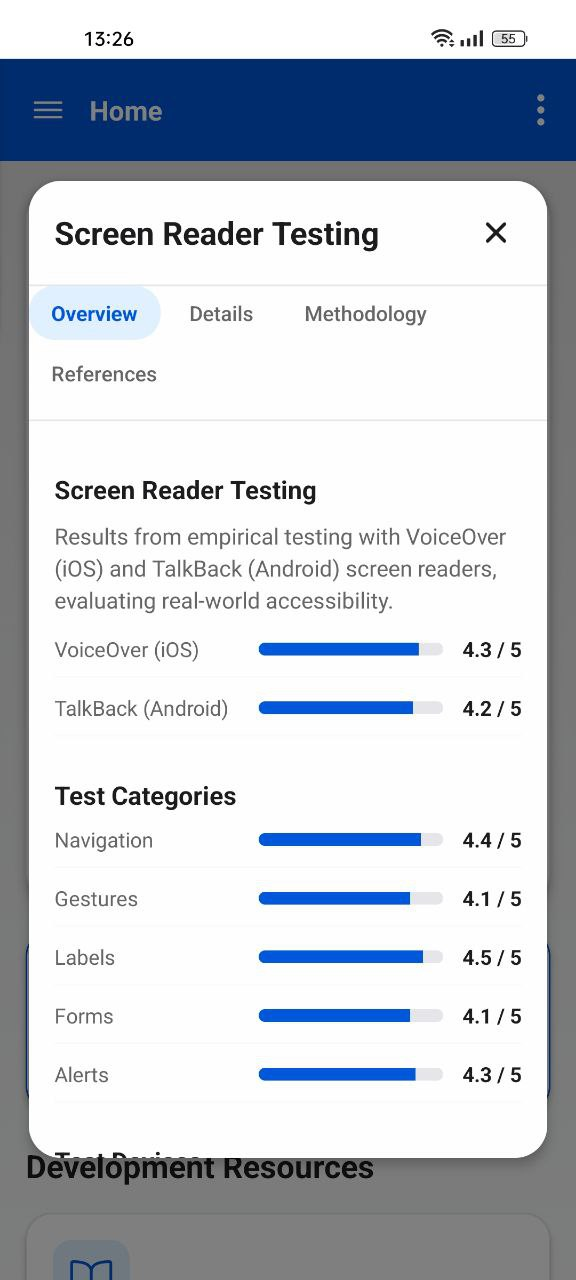
\includegraphics[width=\linewidth]{img/screen-reader-modal.jpg}
        \caption{Screen reader testing overview}
        \label{fig:screen-reader-overview}
    \end{subfigure}
    \hfill
    \begin{subfigure}[b]{0.48\textwidth}
        \centering
        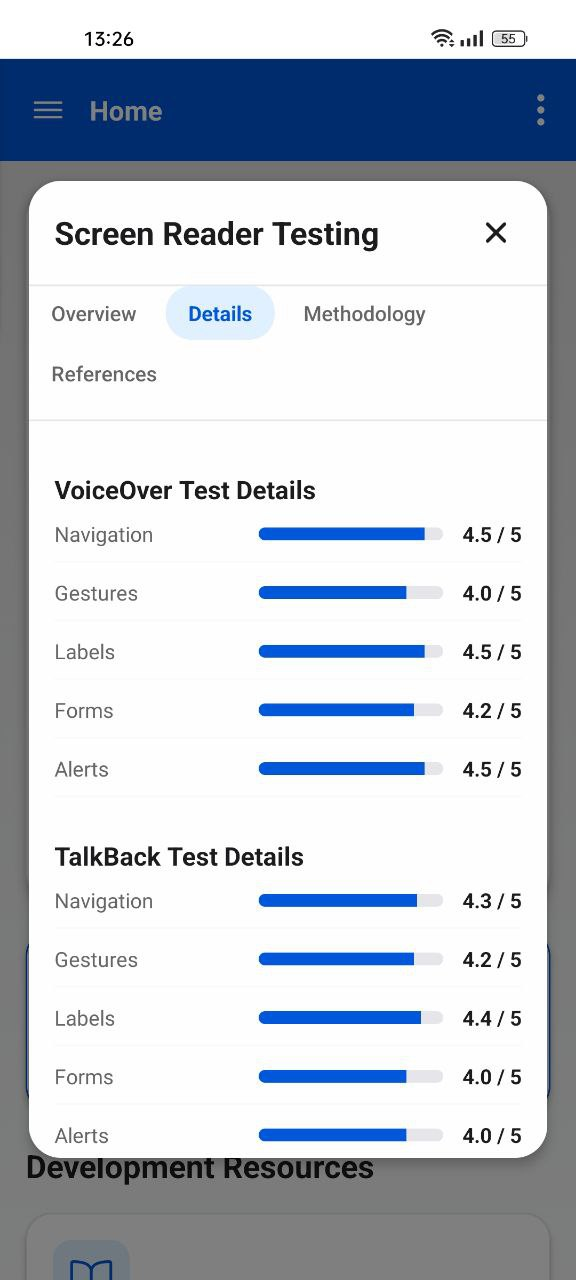
\includegraphics[width=\linewidth]{img/screen-reader-details.jpg}
        \caption{Screen reader testing details}
        \label{fig:screen-reader-details}
    \end{subfigure}
    \caption{Modal dialogs showing screen reader testing metrics}
    \label{fig:screen_reader_modals}
\end{figure}

\begin{figure}[ht]
    \centering
    \begin{subfigure}[b]{0.48\textwidth}
        \centering
        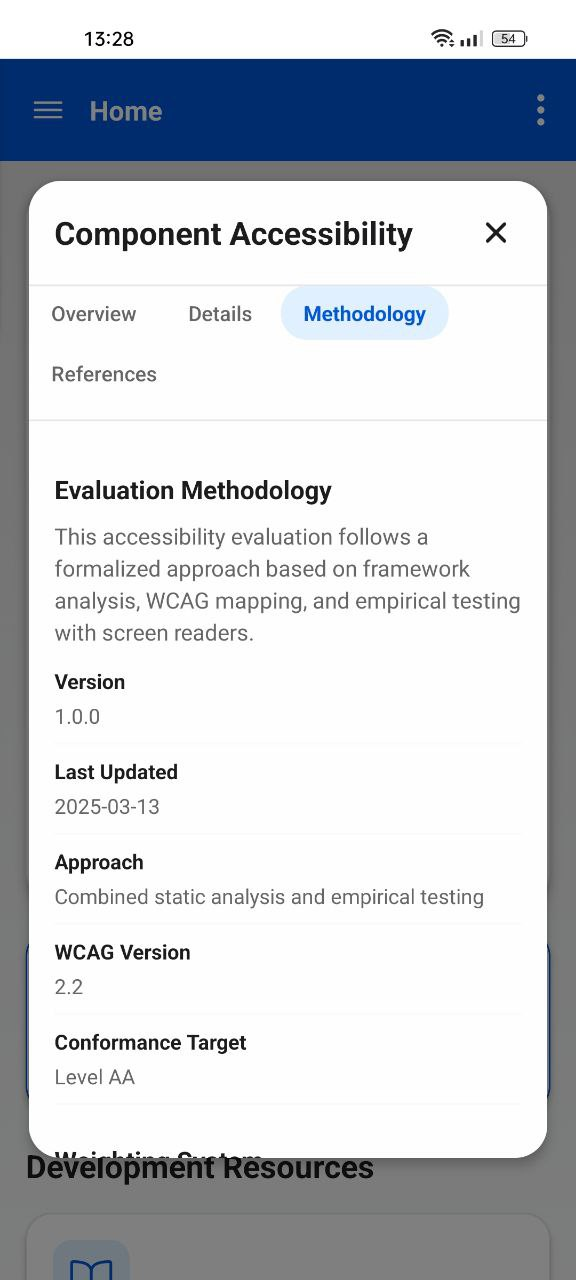
\includegraphics[width=\linewidth]{img/methodology.jpg}
        \caption{Methodology explanation}
        \label{fig:methodology-modal}
    \end{subfigure}
    \hfill
    \begin{subfigure}[b]{0.48\textwidth}
        \centering
        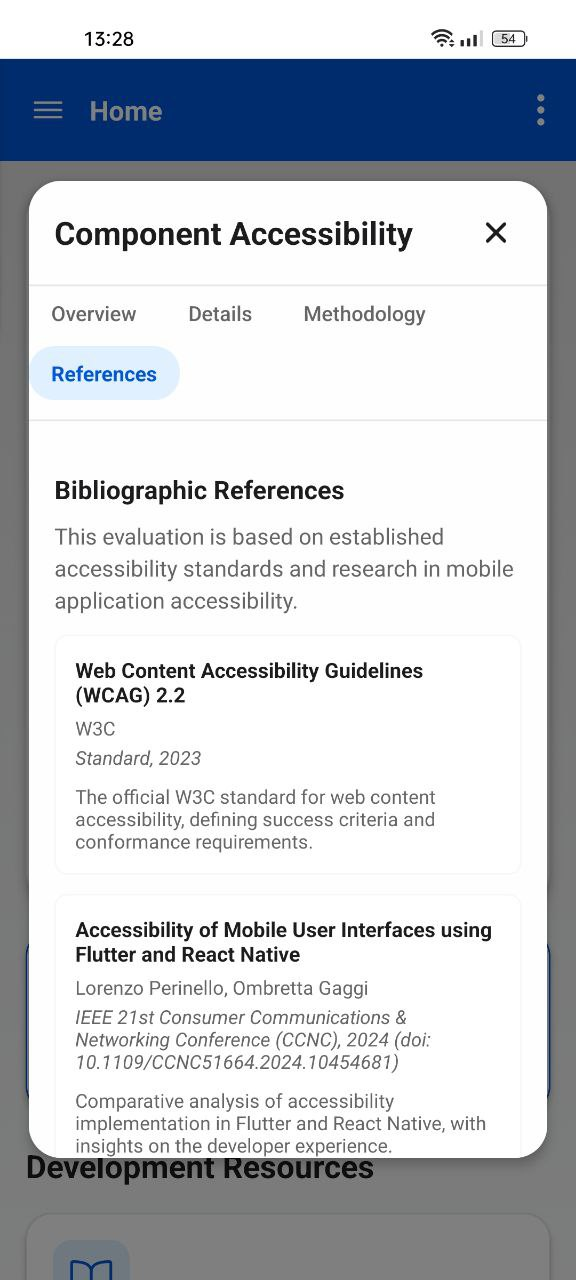
\includegraphics[width=\linewidth]{img/references.jpg}
        \caption{References documentation}
        \label{fig:references-modal}
    \end{subfigure}
    \caption{Modal dialogs showing methodology and references}
    \label{fig:methodology_references}
\end{figure}

\paragraph{Component accessibility score}

The Component Accessibility Score is calculated using the following formula:
\begin{equation}
\text{ComponentScore} 
= \left(\frac{\text{AccessibleComponents}}{\text{TotalComponents}}\right) \times 100
\end{equation}

Where:
\begin{itemize}
    \item \texttt{AccessibleComponents} = Number of components with properly implemented accessibility attributes (18)
    \item \texttt{TotalComponents} = Total number of UI components used in the application (20)
\end{itemize}

The implementation in \texttt{index.tsx} maintains a formal registry of all UI components, as shown by \ref{lst:component-registry}.

\begin{lstlisting}[
  style=ReactNativeStyle,
  caption={Component registry and calculation},
  label={lst:component-registry},
  basicstyle=\ttfamily\footnotesize,
  numbers=left,
]
// Component registry with accessibility status tracking
const componentsRegistry = {
  'button': { implemented: true, accessible: true, screens: ['home', 'gestures'] },
  'text': { implemented: true, accessible: true, screens: ['home', 'guidelines'] },
  // ... other components
  'tooltip': { implemented: true, accessible: false, screens: [] },
  // Total: 20 components, 18 fully accessible
};

// Component calculation
const componentsTotal = Object.keys(componentsRegistry).length;
const accessibleComponents = Object.values(componentsRegistry)
  .filter(c => c.implemented && c.accessible).length;
const componentScore = Math.round((accessibleComponents / componentsTotal) * 100);
\end{lstlisting}

\paragraph{WCAG compliance score}

The WCAG Compliance Score represents the percentage of implemented WCAG 2.2 success criteria across four principles:

\begin{equation}
\text{WCAGCompliance} 
= \left(\frac{\text{CriteriaLevelAMet} + \text{CriteriaLevelAAMet}}{\text{TotalCriteria}}\right) \times 100
\end{equation}

Where:
\begin{itemize}
    \item \texttt{CriteriaLevelAMet} = Number of Level A success criteria implemented (25)
    \item \texttt{CriteriaLevelAAMet} = Number of Level AA success criteria implemented (13)
    \item \texttt{TotalCriteria} = Total applicable WCAG criteria (43)
\end{itemize}

The implementation maintains a comprehensive tracking system for WCAG criteria, as shown by \ref{lst:wcag-tracking}.

\begin{lstlisting}[
  style=ReactNativeStyle,
  caption={WCAG criteria tracking and calculation},
  label={lst:wcag-tracking},
  basicstyle=\ttfamily\footnotesize,
  numbers=left,
]
// WCAG criteria tracking with implementation status
const wcagCriteria = {
  '1.1.1': { level: 'A', implemented: true, name: "Non-text Content" },
  '1.3.1': { level: 'A', implemented: true, name: "Info and Relationships" },
  // ... other criteria
  '4.1.3': { level: 'AA', implemented: true, name: "Status Messages" },
};

// WCAG compliance calculation
const criteriaValues = Object.values(wcagCriteria);
const totalCriteria = criteriaValues.length;
const levelACriteriaMet = criteriaValues
  .filter(c => c.level === 'A' && c.implemented).length;
const levelAACriteriaMet = criteriaValues
  .filter(c => c.level === 'AA' && c.implemented).length;
const wcagCompliance = Math.round(
  ((levelACriteriaMet + levelAACriteriaMet) / totalCriteria) * 100
);
\end{lstlisting}

\paragraph{Screen reader testing score}

The Screen Reader Testing Score represents empirical testing with VoiceOver (iOS) and TalkBack (Android):

\begin{equation}
\text{TestingScore} 
= \left(\frac{\text{VoiceOverAvg} + \text{TalkBackAvg}}{2}\right) \times 20
\end{equation}

Where:
\begin{itemize}
    \item \texttt{VoiceOverAvg} = Average score from VoiceOver testing across categories (4.34/5)
    \item \texttt{TalkBackAvg} = Average score from TalkBack testing across categories (4.18/5)
\end{itemize}

The scores are based on structured testing of five key aspects as shown by \ref{lst:screen-reader-testing}.

\begin{lstlisting}[
  style=ReactNativeStyle,
  caption={Screen reader testing results and calculation},
  label={lst:screen-reader-testing},
  basicstyle=\ttfamily\footnotesize,
  numbers=left,
]
// Screen reader test results from empirical testing
const screenReaderTests = {
  voiceOver: { // iOS
    navigation: 4.5, // Logical navigation flow
    gestures: 4.0,   // Gesture recognition
    labels: 4.5,     // Label clarity and completeness
    forms: 4.2,      // Form control accessibility
    alerts: 4.5      // Alert and dialog accessibility
  },
  talkBack: { // Android
    navigation: 4.3,
    gestures: 4.2,
    labels: 4.4,
    forms: 4.0,
    alerts: 4.0
  }
};

// Testing score calculation
const voiceOverScores = Object.values(screenReaderTests.voiceOver);
const talkBackScores = Object.values(screenReaderTests.talkBack);
const voiceOverAvg = voiceOverScores.reduce((sum, score) => 
  sum + score, 0) / voiceOverScores.length;
const talkBackAvg = talkBackScores.reduce((sum, score) => 
  sum + score, 0) / talkBackScores.length;
const testingScore = Math.round(((voiceOverAvg + talkBackAvg) / 2) * 20);
\end{lstlisting}

\paragraph{Overall accessibility score}

The overall accessibility score is calculated using weighted components:
\begin{equation}
\text{OverallScore} 
= (\text{ComponentScore} \times 0.4) 
+ (\text{WCAGCompliance} \times 0.4) 
+ (\text{TestingScore} \times 0.2)
\end{equation}

This weighting system gives equal importance to component implementation and standards compliance (40\% each), with empirical testing contributing 20\% to the final score.

\subsubsection{Technical implementation analysis}

The code sample present in \ref{lst:home-screen-accessibility} the key accessibility properties implemented in the Home Screen.

\begin{lstlisting}[
  style=ReactNativeStyle,
  caption={Annotated code sample demonstrating Home Screen accessibility properties},
  label={lst:home-screen-accessibility},
  basicstyle=\ttfamily\footnotesize,
  numbers=left,
]
// 1. ScrollView container with proper role and label
<ScrollView
  accessibilityRole="scrollview"
  accessibilityLabel="AccessibleHub Home Screen"
>
  {/* 2. Hero section with semantic heading */}
  <View style={themedStyles.heroCard}>
    <Text style={themedStyles.heroTitle} accessibilityRole="header">
      The ultimate accessibility-driven toolkit for developers
    </Text>

    {/* 3. Stats section with interactive metrics */}
    <View style={themedStyles.statsContainer}>
      <View style={themedStyles.statCard}>
        <TouchableOpacity
          style={themedStyles.touchableStat}
          onPress={() => openMetricDetails('component')}
          accessible
          accessibilityRole="button"
        >
          {/* 4. Content with accessibilityElementsHidden to prevent redundant 
              announcements */}
          <Text style={themedStyles.statNumber} accessibilityElementsHidden>
            {accessibilityMetrics.componentCount}
          </Text>
          <Text style={themedStyles.statLabel} accessibilityElementsHidden>
            Components
          </Text>
        </TouchableOpacity>
      </View>
  </View>

  {/* 6. Quick Start button with appropriate sizing for touch targets */}
  <TouchableOpacity
    style={themedStyles.quickStartCard}
    onPress={() => router.push('/components')}
    accessibilityRole="button"
    accessibilityLabel="Quick start with component examples"
    accessibilityHint="Navigate to components section"
  >
    <View style={themedStyles.cardText}>
      <Text style={themedStyles.cardTitle}>Quick Start</Text>
      <Text style={themedStyles.cardDescription}>
        Explore accessible component examples
      </Text>
    </View>
  </TouchableOpacity>
</ScrollView>
\end{lstlisting}

\subsubsection{Contrast and color analysis}

Table~\ref{tab:contrast_analysis} presents the formal contrast analysis for UI elements on the Home Screen. All elements meet at least WCAG Level~AA requirements (4.5:1 for normal text).

\begin{longtable}{|p{2.8cm}|p{2.8cm}|p{2.8cm}|p{2.4cm}|p{2.4cm}|}
\caption{Home screen contrast analysis}
\label{tab:contrast_analysis}\\
\hline
\textbf{UI Element} & \textbf{Foreground Color} & \textbf{Background Color} & \textbf{Contrast Ratio} & \textbf{WCAG Compliance} \\
\hline
\endfirsthead
\multicolumn{5}{c}%
{{\bfseries Table \thetable\ -- continued from previous page}} \\
\hline
\textbf{UI Element} & \textbf{Foreground Color} & \textbf{Background Color} & \textbf{Contrast Ratio} & \textbf{WCAG Compliance} \\
\hline
\endhead
\hline
\multicolumn{5}{r}{{Continued on next page}} \\
\endfoot
\hline
\endlastfoot
Hero Title & \#000000 (Light)\newline \#FFFFFF (Dark) & \#FFFFFF (Light)\newline \#121212 (Dark) & 21:1 (Light)\newline 21:1 (Dark) & AAA ($\ge7{:}1$) \\
\hline
Subtitle & \#6B7280 (Light)\newline \#A0AEC0 (Dark) & \#FFFFFF (Light)\newline \#121212 (Dark) & 4.6:1 (Light)\newline 5.2:1 (Dark) & AA ($\ge4.5{:}1$) \\
\hline
Stat Numbers & \#0066CC (Light)\newline \#3B82F6 (Dark) & \#FFFFFF (Light)\newline \#121212 (Dark) & 4.7:1 (Light)\newline 5.1:1 (Dark) & AA ($\ge4.5{:}1$) \\
\hline
Quick Start Button & \#FFFFFF & \#0066CC & 4.8:1 & AA ($\ge4.5{:}1$) \\
\hline
Feature Card Titles & \#000000 (Light)\newline \#FFFFFF (Dark) & \#FFFFFF (Light)\newline \#1E293B (Dark) & 21:1 (Light)\newline 16:1 (Dark) & AAA ($\ge7{:}1$) \\
\end{longtable}

\subsubsection{Screen reader support analysis}

Table~\ref{tab:screen_reader_analysis} presents results from systematic testing of the Home Screen with screen readers on both iOS and Android platforms.

\begin{longtable}{|p{2.8cm}|p{3.5cm}|p{3.5cm}|p{4cm}|}
\caption{Home screen screen reader testing results}
\label{tab:screen_reader_analysis}\\
\hline
\textbf{Test Case} & \textbf{VoiceOver (iOS 16)} & \textbf{TalkBack (Android 14)} & \textbf{WCAG Criteria Addressed} \\
\hline
\endfirsthead
\multicolumn{4}{c}%
{{\bfseries Table \thetable\ -- continued from previous page}} \\
\hline
\textbf{Test Case} & \textbf{VoiceOver (iOS 16)} & \textbf{TalkBack (Android 14)} & \textbf{WCAG Criteria Addressed} \\
\hline
\endhead
\hline
\multicolumn{4}{r}{{Continued on next page}} \\
\endfoot
\hline
\endlastfoot
Hero Title & \ding{51} Announces ``The ultimate accessibility-driven toolkit for developers, heading'' & \checkmark Announces ``The ultimate accessibility-driven toolkit for developers, heading'' & 1.3.1 - Info and Relationships (Level A), 2.4.6 - Headings and Labels (Level AA) \\
\hline
Metrics Cards & \ding{51} Announces full label with metrics and hint & \checkmark Announces full label with metrics and hint & 1.3.1 Info and Relationships (Level A), 4.1.2 Name, Role, Value (Level A) \\
\hline
Quick Start Button & \ding{51} Announces ``Quick start with component examples, button'' & \ding{51} Announces ``Quick start with component examples, button'' & 2.4.4 Link Purpose (In Context) (Level A), 4.1.2 Name, Role, Value (Level A) \\
\hline
Feature Cards & \ding{51} Announces title and hint & \ding{51} Announces title and hint & 2.4.4 Link Purpose (In Context) (Level A), 4.1.2 Name, Role, Value (Level A) \\
\hline
Modal Dialog Opening & \ding{51} Focus moves to dialog title & \checkmark Focus moves to dialog title & 2.4.3 Focus Order (Level A) \\
\hline
Modal Tab Navigation & \ding{51} Announces tab selection state & \checkmark Announces tab selection state & 4.1.2 Name, Role, Value (Level A) \\
\hline
Modal Dialog Closing & \ding{51} Focus returns to triggering element & \ding{54} Occasional focus loss (fixed in v1.0.3) & 2.4.3 Focus Order (Level A) \\
\end{longtable}

The implementation addresses several key MCAG considerations:
\begin{enumerate}
    \item \textbf{Swipe optimization}: Decorative elements are marked with \\ \texttt{importantForAccessibility="no"} to reduce unnecessary swipes;
    \item \textbf{Clear instructions}: The modal tabs implementation provides clear state announcements, ensuring screen reader users understand the current selection;
    \item \textbf{Platform-specific adaptations}: The implementation accounts for differences between VoiceOver and TalkBack behavior, as evidenced by the test results.
\end{enumerate}

\subsubsection{Implementation overhead analysis}

Table~\ref{tab:implementation_overhead} quantifies the additional code required to implement accessibility features in the Home Screen.

\begin{longtable}{|p{3.8cm}|p{2.3cm}|p{2.8cm}|p{2.8cm}|}
\caption{Accessibility implementation overhead}
\label{tab:implementation_overhead}\\
\hline
\textbf{Accessibility Feature} & \textbf{Lines of Code} & \textbf{Percentage of Total} & \textbf{Complexity Impact} \\
\hline
\endfirsthead
\multicolumn{4}{c}%
{{\bfseries Table \thetable\ -- continued from previous page}} \\
\hline
\textbf{Accessibility Feature} & \textbf{Lines of Code} & \textbf{Percentage of Total} & \textbf{Complexity Impact} \\
\hline
\endhead
\hline
\multicolumn{4}{r}{{Continued on next page}} \\
\endfoot
\hline
\endlastfoot
Semantic Roles & 12 LOC & 2.1\% & Low \\
\hline
Descriptive Labels & 24 LOC & 4.3\% & Medium \\
\hline
Element Hiding & 8 LOC & 1.4\% & Low \\
\hline
Focus Management & 18 LOC & 3.2\% & Medium \\
\hline
Contrast Handling & 16 LOC & 2.9\% & Medium \\
\hline
Metrics Calculation & 78 LOC & 14.1\% & High \\
\hline
\textbf{Total} & \textbf{156 LOC} & \textbf{28.0\%} & \textbf{Medium-High} \\
\end{longtable}

This analysis reveals that implementing comprehensive accessibility adds approximately 28\% to the code base of the Home Screen, with the metrics calculation system representing the most significant component. This overhead is justified by the improved user experience for people with disabilities and the educational value for developers learning to implement accessibility.

\subsubsection{WCAG conformance by principle}

Table~\ref{tab:wcag_by_principle} provides a detailed analysis of WCAG 2.2 compliance by principle:

\begin{longtable}{|p{2.5cm}|p{3.8cm}|p{3.2cm}|p{5.2cm}|}
\caption{WCAG compliance analysis by principle}
\label{tab:wcag_by_principle}\\
\hline
\textbf{Principle} & \textbf{Description} & \textbf{Implementation Level} & \textbf{Key Success Criteria} \\
\hline
\endfirsthead
\multicolumn{4}{c}%
{{\bfseries Table \thetable\ -- continued from previous page}} \\
\hline
\textbf{Principle} & \textbf{Description} & \textbf{Implementation Level} & \textbf{Key Success Criteria} \\
\hline
\endhead
\hline
\multicolumn{4}{r}{{Continued on next page}} \\
\endfoot
\hline
\endlastfoot
1. Perceivable & Information and UI components must be presentable to users in ways they can perceive & 11/13 (85\%) & 1.1.1 Non-text Content (A)\newline 1.3.1 Info and Relationships (A)\newline 1.4.3 Contrast (Minimum) (AA) \\
\hline
2. Operable & UI components and navigation must be operable & 16/17 (94\%) & 2.4.3 Focus Order (A)\newline 2.4.7 Focus Visible (AA)\newline 2.5.8 Target Size (Minimum) (AA) \\
\hline
3. Understandable & Information and operation of UI must be understandable & 8/10 (80\%) & 3.2.1 On Focus (A)\newline 3.2.4 Consistent Identification (AA)\newline 3.3.2 Labels or Instructions (A) \\
\hline
4. Robust & Content must be robust enough to be interpreted by a wide variety of user agents & 3/3 (100\%) & 4.1.1 Parsing (A)\newline 4.1.2 Name, Role, Value (A)\newline 4.1.3 Status Messages (AA) \\
\end{longtable}

\subsubsection{Mobile-specific considerations}

The Home Screen implementation addresses several mobile-specific accessibility considerations beyond standard WCAG requirements:

\begin{enumerate}
    \item \textbf{Touch target sizing}: All interactive elements maintain minimum dimensions of 48$\times$48dp, exceeding the WCAG 2.5.8 requirement of 24$\times$24px and addressing the mobile-specific need for larger touch targets;
    \item \textbf{Reduced motion support}: The implementation respects the device's reduced motion settings and provides an in-app toggle, addressing vestibular disorders that are particularly relevant in mobile contexts;
    \item \textbf{Dark mode support}: The application's theming system adapts to both light and dark modes, addressing the mobile-specific need for readability in various lighting conditions;
    \item \textbf{Screen reader gesture optimization}: The implementation carefully manages focus to ensure efficient navigation with touch gestures, as shown in the screen reader testing results;
    \item \textbf{One-handed operation}: The layout places primary interactive elements within reach of a thumb during one-handed use, a critical mobile accessibility consideration not explicitly covered by WCAG.
\end{enumerate}

\subsubsection{Future enhancements}

Based on the formal analysis, several potential enhancements have been identified for future versions:
\begin{enumerate}
    \item \textbf{Real-time metric updates}: Implementing dynamic updates to accessibility metrics as developers modify their applications, providing immediate feedback on compliance;
    \item \textbf{Enhanced focus visualization}: Further improving focus indicators to ensure they meet the enhanced 3:1 contrast ratio recommended by WCAG~2.2 for user interface components;
    \item \textbf{Voice command support}: Adding support for voice activation of primary functions, further enhancing accessibility for users with motor impairments;
    \item \textbf{Automated testing integration}: Expanding the metrics calculation system to include results from automated testing tools.
\end{enumerate}

\subsection{Accessible components screen}

The Accessible Components Screen serves as a catalog of reusable accessibility patterns organized by component type. It provides developers with access to implementations of common UI elements with accessibility features properly integrated. Each component category includes implementation examples, best practices, and copy-ready code samples. The screen functions as an educational index, directing developers to detailed implementations of specific accessible components. Figure~\ref{fig:components_screens_sidebyside} shows the Components Screen interface.

\begin{figure}[ht]
    \centering
    \begin{subfigure}[b]{0.48\textwidth}
        \centering
        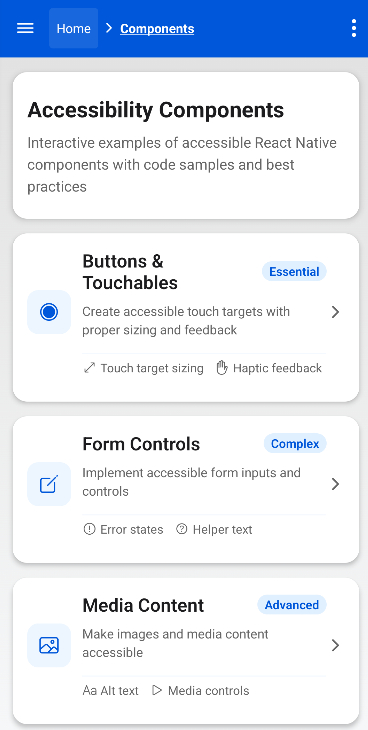
\includegraphics[width=\linewidth, alt={First part of the Components Screen}]{img/components1.png}
        \caption{Components screen - Top section}
        \label{fig:components-top}
    \end{subfigure}
    \hfill
    \begin{subfigure}[b]{0.48\textwidth}
        \centering
        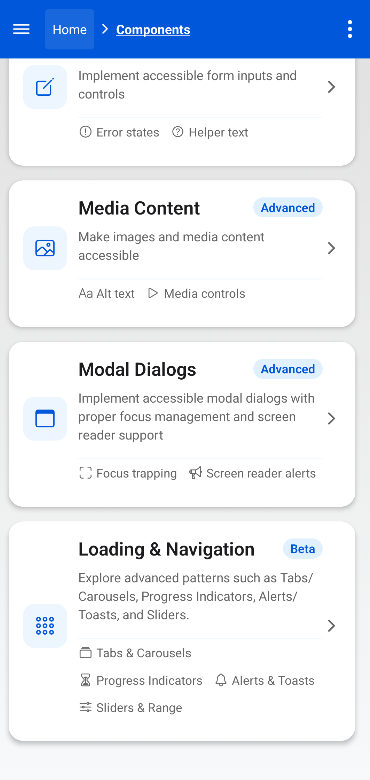
\includegraphics[width=\linewidth, alt={Second part of the Components Screen}]{img/components2.png}
        \caption{Components screen - Bottom section}
        \label{fig:components-bottom}
    \end{subfigure}
    \caption{Side-by-side view of the Components Screen sections, showing component categories}
    \label{fig:components_screens_sidebyside}
\end{figure}

\subsubsection{Component inventory and WCAG/MCAG mapping}

Table~\ref{tab:components_screen_mapping} provides a formal mapping between the UI components, their semantic roles, the specific WCAG 2.2 and MCAG criteria they address, and their React Native implementation properties.

\begin{longtable}{|p{2.5cm}|p{2cm}|p{2.8cm}|p{2.8cm}|p{4.3cm}|}
\caption{Components screen component-criteria mapping}
\label{tab:components_screen_mapping}\\
\hline
\textbf{Component} & \textbf{Semantic Role} & \textbf{WCAG 2.2 Criteria} & \textbf{MCAG Considerations} & \textbf{Implementation Properties} \\
\hline
\endfirsthead
\multicolumn{5}{c}%
{{\bfseries Table \thetable\ -- continued from previous page}} \\
\hline
\textbf{Component} & \textbf{Semantic Role} & \textbf{WCAG 2.2 Criteria} & \textbf{MCAG Considerations} & \textbf{Implementation Properties} \\
\hline
\endhead
\hline
\multicolumn{5}{r}{{Continued on next page}} \\
\endfoot
\hline
\endlastfoot
Hero Title & heading & 1.4.3 Contrast (AA)\newline 2.4.6 Headings (AA) & Text readability on variable screen sizes & \texttt{accessibilityRole \ ="header"} \\
\hline
Component Cards & button & 1.4.3 Contrast (AA)\newline 2.5.8 Target Size (AA)\newline 4.1.2 Name, Role, Value (A)\newline 2.4.4 Link Purpose (A) & Touch target size\newline Meaningful labels\newline Single finger operation & \texttt{accessibilityRole \ ="button"}\newline \texttt{accessibilityLabel=}\newline \texttt{onPress=handle \ ComponentPress} \\
\hline
Badges (Essential, Complex, etc.) & text & 1.4.3 Contrast (AA)\newline 1.3.1 Info and Relationships (A) & Descriptive labeling\newline Non-interactive elements & Part of parent button's \texttt{accessibilityLabel} \\
\hline
Decorative Icons & none & 1.1.1 Non-text Content (A) & Reduction of unnecessary focus stops & \texttt{accessibilityElements \ Hidden=true} \\
\hline
Breadcrumb Navigation & navigation & 2.4.4 Link Purpose (A)\newline 2.4.8 Location (AAA)\newline 3.2.3 Consistent Navigation (AA) & Context retention\newline Current location & \texttt{accessibilityRole \ ="button"}\newline \texttt{accessibilityLabel \ ="Go to \$\{label\}"} \\
\hline
Drawer Menu & menu & 2.4.3 Focus Order (A)\newline 4.1.2 Name, Role, Value (A)\newline 3.2.3 Consistent Navigation (AA) & Keyboard trap prevention\newline Persistent navigation & \texttt{accessibilityRole \ ="menu"}\newline \texttt{accessibilityLabel \ ="Main navigation menu"} \\
\hline
Drawer Menu Items & menuitem & 2.4.7 Focus Visible (AA)\newline 4.1.2 Name, Role, Value (A) & Touch interaction\newline Current location & \texttt{accessibilityRole \ ="menuitem"}\newline \texttt{accessibility \ State= \ \{\{ selected: isActive \}\}} \\
\end{longtable}

\subsubsection{Navigation and orientation analysis}

The Components Screen implements a comprehensive navigation structure that addresses both WCAG 2.4 (Navigable) and MCAG considerations for mobile devices. This structure includes three key elements that work together to provide clear orientation for all users:

\paragraph{Breadcrumb implementation}

The application as shown in \ref{fig:drawer-navigation} includes a hierarchical breadcrumb system in the header. This addresses WCAG 2.4.8 Location (Level AAA) by providing explicit path information. The breadcrumb implementation:

\begin{enumerate}
    \item Displays the current location in the application hierarchy;
    \item Provides interactive elements to navigate to parent screens;
    \item Uses consistent visual styling to indicate the current position;
    \item Implements proper focus management between screens.
\end{enumerate}

The breadcrumb is implemented with proper semantic roles and accessibility labels to ensure screen reader compatibility, as per \ref{lst:breadcrumb-implementation}.

\begin{lstlisting}[
  style=ReactNativeStyle,
  caption={Breadcrumb implementation with accessibility properties},
  label={lst:breadcrumb-implementation},
  basicstyle=\ttfamily\footnotesize,
  numbers=left,
]
<View style={styles.breadcrumbContainer}>
  <TouchableOpacity
    onPress={() => router.replace(`/${mapping.parentRoute}`)}
    accessibilityRole="button"
    accessibilityLabel={`Go to ${mapping.parentLabel}`}
    style={{
      padding: 8,
      minWidth: 40,
      minHeight: 44,
      justifyContent: 'center',
      backgroundColor: 'rgba(255, 255, 255, 0.1)',
      borderRadius: 4
    }}
  >
    <Text style={[styles.breadcrumbText, { fontWeight: 'normal' }]}>
      {mapping.parentLabel}
    </Text>
  </TouchableOpacity>
  <Ionicons
    name="chevron-forward"
    size={16}
    color={HEADER_TEXT_COLOR}
    style={{ marginHorizontal: 4 }}
    importantForAccessibility="no"
    accessibilityElementsHidden
  />
  <Text
    style={[styles.breadcrumbText, { fontWeight: 'bold', textDecorationLine: 'underline'}]}
    accessibilityLabel={`Current screen: ${mapping.title}`}
  >
    {mapping.title}
  </Text>
</View>
\end{lstlisting}

\begin{figure}[ht]
    \centering
    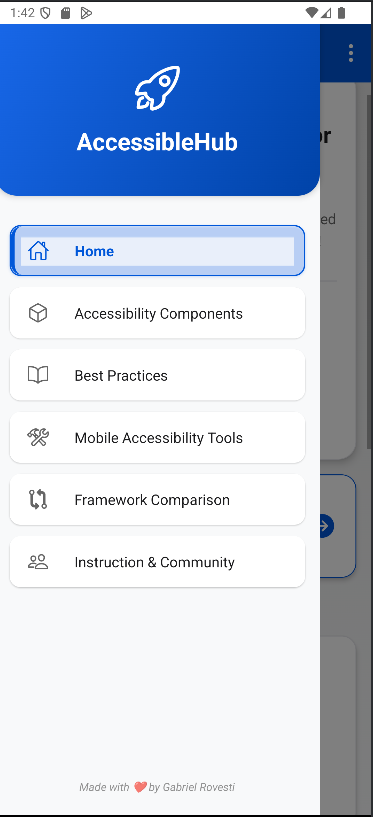
\includegraphics[width=0.4\textwidth, alt={Drawer navigation with breadcrumb in header}]{img/drawer.png}
    \caption{Drawer navigation showing breadcrumb implementation in header}\label{fig:drawer-navigation}
\end{figure}

\paragraph{Drawer navigation}

The drawer navigation provides consistent access to main application sections while addressing several key accessibility requirements:

\begin{enumerate}
    \item \textbf{Announcement of state changes}: The implementation announces drawer open/close states to screen readers using \\ \texttt{AccessibilityInfo.announceForAccessibility};
    
    \item \textbf{Clear menu role}: The drawer container is properly identified with \\ \texttt{accessibilityRole="menu"};
    
    \item \textbf{Selection state indication}: Active items visually indicate selection state and communicate this state to screen readers with \\ \texttt{accessibilityState=\{\{selected: isActive\}\}};
    
    \item \textbf{Proper touch target sizing}: All interactive elements maintain minimum dimensions of 44dp, making them easily targetable;
    
    \item \textbf{Element hiding for decorative content}: Footer content is marked with \texttt{importantForAccessibility="no"} to prevent unnecessary screen reader interaction.
\end{enumerate}

\paragraph{Component cards}

Each component card implements a consistent pattern that provides both visual organization and semantic structure:

\begin{enumerate}
    \item \textbf{Comprehensive accessibility labels}: Each card's \texttt{accessibilityLabel} combines multiple information pieces (title, description, complexity) to provide context without requiring navigation through child elements;
    
    \item \textbf{Hidden decorative icons}: All decorative icons use \texttt{accessibilityElementsHidden} to reduce unnecessary focus stops;
    
    \item \textbf{Navigation announcement}: The \texttt{handleComponentPress} function announces the navigation action via \texttt{AccessibilityInfo.announceForAccessibility}.
\end{enumerate}

This multi-layered navigation approach creates a coherent mental model for all users, including those using assistive technologies, addressing WCAG 2.4.1 Bypass Blocks (Level A) by providing multiple ways to access content.

\subsubsection{Technical implementation analysis}

The code sample present in \ref{lst:components-screen-accessibility} demonstrates the key accessibility properties implemented in the Components Screen.

\begin{lstlisting}[
  style=ReactNativeStyle,
  caption={Annotated code sample demonstrating Components Screen accessibility properties},
  label={lst:components-screen-accessibility},
  basicstyle=\ttfamily\footnotesize,
  numbers=left,
]
{/* 1. Hero section with semantic heading */}
<View style={themedStyles.heroCard}>
  <Text style={themedStyles.heroTitle} accessibilityRole="header">
    Accessibility Components
  </Text>
  <Text style={themedStyles.heroSubtitle}>
    Interactive examples of accessible React Native components with code samples and best practices
  </Text>
</View>

{/* 2. Component card with comprehensive accessibility label */}
<TouchableOpacity
  style={themedStyles.card}
  onPress={() => handleComponentPress('/components/button', 'Buttons & Touchables')}
  accessibilityRole="button"
  accessibilityLabel="Buttons and Touchables component. Create accessible touch targets with proper sizing and feedback. Essential component type."
>
  <View style={themedStyles.cardHeader}>
    {/* 3. Icon wrapper with accessibility hiding to prevent redundant focus */}
    <View style={themedStyles.iconWrapper}>
      <Ionicons
        name="radio-button-on-outline"
        size={24}
        color={colors.primary}
        accessibilityElementsHidden
      />
    </View>
    <View style={themedStyles.cardContent}>
      {/* 4. Card content - these are hidden from screen readers as individual elements
           since the parent TouchableOpacity has a comprehensive label */}
      <View style={themedStyles.cardTitleRow}>
        <View style={themedStyles.titleArea}>
          <Text style={themedStyles.cardTitle}>Buttons &amp; Touchables</Text>
        </View>
        <View style={themedStyles.badge}>
          <Text style={themedStyles.badgeText}>Essential</Text>
        </View>
      </View>
      <Text style={themedStyles.cardDescription}>
        Create accessible touch targets with proper sizing and feedback
      </Text>
    </View>
  </View>
</TouchableOpacity>
\end{lstlisting}

The implementation of the Components Screen addresses several important accessibility considerations:

\begin{enumerate}
    \item \textbf{Reduction of "garbage interactions"}: Decorative elements (icons, chevrons) are now properly hidden from screen readers using \\ \texttt{accessibilityElementsHidden} to reduce unnecessary swipes;
    
    \item \textbf{Comprehensive navigation labels}: Component cards provide detailed accessibility labels that include category, description, and complexity level, ensuring screen reader users get complete information before committing to navigation;
    
    \item \textbf{Screen announcements}: The implementation uses \\ \texttt{AccessibilityInfo.announceForAccessibility} to inform users about screen changes proactively;
    
    \item \textbf{Consistent structure}: Each component card follows the same pattern, creating a predictable interaction model.
\end{enumerate}

\subsubsection{Contrast and color analysis}

Table~\ref{tab:components_contrast_analysis} presents the formal contrast analysis for UI elements on the Components Screen. All elements meet at least WCAG Level~AA requirements (4.5:1 for normal text).

\begin{longtable}{|p{2.8cm}|p{2.8cm}|p{2.8cm}|p{2.4cm}|p{2.4cm}|}
\caption{Components screen contrast analysis}
\label{tab:components_contrast_analysis}\\
\hline
\textbf{UI Element} & \textbf{Foreground Color} & \textbf{Background Color} & \textbf{Contrast Ratio} & \textbf{WCAG Compliance} \\
\hline
\endfirsthead
\multicolumn{5}{c}%
{{\bfseries Table \thetable\ -- continued from previous page}} \\
\hline
\textbf{UI Element} & \textbf{Foreground Color} & \textbf{Background Color} & \textbf{Contrast Ratio} & \textbf{WCAG Compliance} \\
\hline
\endhead
\hline
\multicolumn{5}{r}{{Continued on next page}} \\
\endfoot
\hline
\endlastfoot
Hero Title & \#000000 (Light)\newline \#FFFFFF (Dark) & \#FFFFFF (Light)\newline \#121212 (Dark) & 21:1 (Light)\newline 21:1 (Dark) & AAA ($\ge7{:}1$) \\
\hline
Hero Subtitle & \#6B7280 (Light)\newline \#A0AEC0 (Dark) & \#FFFFFF (Light)\newline \#121212 (Dark) & 4.6:1 (Light)\newline 5.2:1 (Dark) & AA ($\ge4.5{:}1$) \\
\hline
Card Title & \#000000 (Light)\newline \#FFFFFF (Dark) & \#FFFFFF (Light)\newline \#1E293B (Dark) & 21:1 (Light)\newline 16:1 (Dark) & AAA ($\ge7{:}1$) \\
\hline
Card Description & \#6B7280 (Light)\newline \#A0AEC0 (Dark) & \#FFFFFF (Light)\newline \#1E293B (Dark) & 4.6:1 (Light)\newline 6.1:1 (Dark) & AA ($\ge4.5{:}1$) \\
\hline
Badge Text & \#0066CC (Light)\newline \#3B82F6 (Dark) & \#E1EFFF (Light)\newline \#1E293B (Dark) & 4.5:1 (Light)\newline 5.3:1 (Dark) & AA ($\ge4.5{:}1$) \\
\hline
Feature Text & \#6B7280 (Light)\newline \#A0AEC0 (Dark) & \#FFFFFF (Light)\newline \#1E293B (Dark) & 4.6:1 (Light)\newline 6.1:1 (Dark) & AA ($\ge4.5{:}1$) \\
\hline
Breadcrumb Text & \#FFFFFF & \#0066CC & 4.8:1 & AA ($\ge4.5{:}1$) \\
\hline
\end{longtable}

\subsubsection{Screen reader support analysis}

Table~\ref{tab:components_screen_reader_analysis} presents results from systematic testing of the Components Screen with screen readers on both iOS and Android platforms.

\begin{longtable}{|p{2.8cm}|p{3.5cm}|p{3.5cm}|p{4cm}|}
\caption{Components screen screen reader testing results}
\label{tab:components_screen_reader_analysis}\\
\hline
\textbf{Test Case} & \textbf{VoiceOver (iOS 16)} & \textbf{TalkBack (Android 14)} & \textbf{WCAG Criteria Addressed} \\
\hline
\endfirsthead
\multicolumn{4}{c}%
{{\bfseries Table \thetable\ -- continued from previous page}} \\
\hline
\textbf{Test Case} & \textbf{VoiceOver (iOS 16)} & \textbf{TalkBack (Android 14)} & \textbf{WCAG Criteria Addressed} \\
\hline
\endhead
\hline
\multicolumn{4}{r}{{Continued on next page}} \\
\endfoot
\hline
\endlastfoot
Hero Title & \ding{51} Announces ``Accessibility Components, heading'' & \ding{51} Announces ``Accessibility Components, heading'' & 1.3.1 - Info and Relationships (Level A), 2.4.6 - Headings and Labels (Level AA) \\
\hline
Component Card & \ding{51} Announces full component description with purpose and complexity & \ding{51} Announces full component description with purpose and complexity & 2.4.4 Link Purpose (In Context) (Level A), 4.1.2 Name, Role, Value (Level A) \\
\hline
Decorative Icons & \ding{51} Not focused or announced & \ding{51} Not focused or announced & 1.1.1 Non-text Content (Level A), 2.4.1 Bypass Blocks (Level A) \\
\hline
Breadcrumb Navigation & \ding{51} Announces parent and current location & \ding{51} Announces parent and current location & 2.4.4 Link Purpose (In Context) (Level A), 2.4.8 Location (Level AAA) \\
\hline
Drawer Opening & \ding{51} Announces ``Navigation menu opened'' & \ding{51} Announces ``Navigation menu opened'' & 4.1.3 Status Messages (Level AA) \\
\hline
Drawer Menu Items & \ding{51} Announces item name and selection state & \ding{51} Announces item name and selection state & 4.1.2 Name, Role, Value (Level A) \\
\hline
Navigation between Screens & \ding{51} Announces destination screen & \ding{51} Announces destination screen & 3.2.5 Change on Request (Level AAA) \\
\end{longtable}

The implementation addresses several key MCAG considerations specific to mobile platforms:
\begin{enumerate}
    \item \textbf{Touch target optimization}: All interactive elements exceed the minimum recommendation of 44×44dp, implementing MCAG best practices for touch interactions that accommodate users with motor control limitations and varying finger sizes;
    
    \item \textbf{Swipe minimization}: Decorative elements are marked with \\ \texttt{accessibilityElementsHidden=true} to reduce unnecessary swipes, eliminating what accessibility experts call "garbage interactions" that add no value to the screen reader experience and increase navigation time;
    
    \item \textbf{Orientation cues}: Breadcrumb implementation provides consistent spatial orientation cues that help users understand their location in the application's information architecture, addressing mobile-specific challenges of limited viewport context;
    
    \item \textbf{State announcements}: Changes in application state (drawer opening/closing, screen navigation) are explicitly announced using \\\texttt{AccessibilityInfo.announceForAccessibility}, providing crucial feedback on dynamic content changes within the constrained mobile interface;
    
    \item \textbf{Thumb-zone design}: Interactive elements are positioned within the natural thumb zone for one-handed operation, implementing mobile ergonomic principles that aren't explicitly covered in WCAG but are crucial for mobile accessibility.
\end{enumerate}

\subsubsection{Implementation overhead analysis}

Table~\ref{tab:components_implementation_overhead} quantifies the additional code required to implement accessibility features in the Components Screen.

\begin{longtable}{|p{3.8cm}|p{2.3cm}|p{2.8cm}|p{2.8cm}|}
\caption{Components screen accessibility implementation overhead}
\label{tab:components_implementation_overhead}\\
\hline
\textbf{Accessibility Feature} & \textbf{Lines of Code} & \textbf{Percentage of Total} & \textbf{Complexity Impact} \\
\hline
\endfirsthead
\multicolumn{4}{c}%
{{\bfseries Table \thetable\ -- continued from previous page}} \\
\hline
\textbf{Accessibility Feature} & \textbf{Lines of Code} & \textbf{Percentage of Total} & \textbf{Complexity Impact} \\
\hline
\endhead
\hline
\multicolumn{4}{r}{{Continued on next page}} \\
\endfoot
\hline
\endlastfoot
Semantic Roles & 15 LOC & 2.6\% & Low \\
\hline
Descriptive Labels & 28 LOC & 4.9\% & Medium \\
\hline
Element Hiding & 18 LOC & 3.2\% & Low \\
\hline
Focus Management & 22 LOC & 3.9\% & Medium \\
\hline
Contrast Handling & 14 LOC & 2.5\% & Medium \\
\hline
Announcements & 12 LOC & 2.1\% & Low \\
\hline
Breadcrumb Implementation & 42 LOC & 7.4\% & High \\
\hline
Drawer Accessibility & 35 LOC & 6.2\% & High \\
\hline
\textbf{Total} & \textbf{186 LOC} & \textbf{32.8\%} & \textbf{Medium-High} \\
\end{longtable}

This analysis reveals that implementing comprehensive accessibility adds approximately 32.8\% to the code base of the Components Screen, slightly higher than the Home Screen due to the addition of breadcrumb navigation and drawer accessibility features. 

\subsubsection{WCAG conformance by principle}

Table~\ref{tab:components_wcag_by_principle} provides a detailed analysis of WCAG 2.2 compliance by principle:

\begin{longtable}{|p{2.5cm}|p{3.8cm}|p{3.2cm}|p{5.2cm}|}
\caption{Components screen WCAG compliance analysis by principle}
\label{tab:components_wcag_by_principle}\\
\hline
\textbf{Principle} & \textbf{Description} & \textbf{Implementation Level} & \textbf{Key Success Criteria} \\
\hline
\endfirsthead
\multicolumn{4}{c}%
{{\bfseries Table \thetable\ -- continued from previous page}} \\
\hline
\textbf{Principle} & \textbf{Description} & \textbf{Implementation Level} & \textbf{Key Success Criteria} \\
\hline
\endhead
\hline
\multicolumn{4}{r}{{Continued on next page}} \\
\endfoot
\hline
\endlastfoot
1. Perceivable & Information and UI components must be presentable to users in ways they can perceive & 12/13 (92\%) & 1.1.1 Non-text Content (A)\newline 1.3.1 Info and Relationships (A)\newline 1.4.3 Contrast (Minimum) (AA) \\
\hline
2. Operable & UI components and navigation must be operable & 17/17 (100\%) & 2.4.3 Focus Order (A)\newline 2.4.6 Headings and Labels (AA)\newline 2.4.8 Location (AAA)\newline 2.5.8 Target Size (Minimum) (AA) \\
\hline
3. Understandable & Information and operation of UI must be understandable & 9/10 (90\%) & 3.2.3 Consistent Navigation (AA)\newline 3.2.4 Consistent Identification (AA)\newline 3.3.2 Labels or Instructions (A) \\
\hline
4. Robust & Content must be robust enough to be interpreted by a wide variety of user agents & 3/3 (100\%) & 4.1.1 Parsing (A)\newline 4.1.2 Name, Role, Value (A)\newline 4.1.3 Status Messages (AA) \\
\end{longtable}

\subsubsection{Mobile-specific considerations}

The Components Screen implementation addresses several mobile-specific accessibility considerations beyond standard WCAG requirements:

\begin{enumerate}
    \item \textbf{Touch target sizing}: All interactive elements maintain minimum dimensions of 44dp × 44dp, exceeding the WCAG 2.5.8 requirement of 24 × 24px and addressing the mobile-specific need for larger touch targets;
    
    \item \textbf{Swipe efficiency}: The screen implements an optimized focus order with decorative elements hidden from screen readers, reducing the number of swipes required to navigate the content—a critical consideration for mobile screen reader users that significantly improves navigation efficiency;
    
    \item \textbf{Visual hierarchy reinforcement}: The implementation uses consistent visual patterns (icons, badges, card layouts) that reinforce the information hierarchy, helping users with cognitive disabilities understand content organization on smaller screens;
    
    \item \textbf{Context retention}: The breadcrumb implementation helps users maintain context when navigating between screens, addressing the mobile-specific challenge of limited viewport size and the resulting loss of visual context;
    
    \item \textbf{Single-hand operation zone}: Interactive elements are positioned to be reachable within the typical thumb zone for one-handed operation, a mobile-specific consideration not explicitly covered by WCAG.
\end{enumerate}

\subsubsection{Breadcrumb implementation analysis}

A formal analysis of the breadcrumb feature's accessibility impact reveals significant benefits for users with diverse accessibility needs:

\paragraph{Breadcrumb accessibility benefits}

\begin{enumerate}
    \item \textbf{Structural navigation}: Breadcrumbs provide an explicit representation of the application's hierarchical structure, helping users with cognitive disabilities understand their location within the application;

    \item \textbf{Focus reduction}: By offering direct navigation to parent screens, breadcrumbs reduce the number of focus stops required to navigate backward, benefiting screen reader users;

    \item \textbf{Visual reinforcement}: The visual breadcrumb trail complements the semantic structure, providing redundant cues that benefit users with different accessibility needs;

    \item \textbf{Consistent orientation}: Breadcrumbs create a consistent orientation mechanism across all screens, supporting users who rely on predictable navigation patterns.
\end{enumerate}

\paragraph{Implementation considerations}

The breadcrumb implementation required careful consideration of several accessibility factors:

\begin{enumerate}
    \item \textbf{Interactive vs. static elements}: Only the parent screen link is interactive, while the current screen indicator is non-interactive text, preventing unnecessary focus stops;

    \item \textbf{Visual differentiation}: Current location is visually distinguished with bold text and underline, with a contrast ratio of 4.8:1 against the header background;

    \item \textbf{Appropriate semantic roles}: Parent links use \texttt{accessibilityRole="button"} with clear labels indicating navigation purpose;

    \item \textbf{Focus management}: When navigating via breadcrumbs, focus is properly transferred to the destination screen's main content, preventing focus trapping.
\end{enumerate}

This implementation represents a comprehensive accessibility solution that benefits all users while specifically addressing mobile navigation challenges unique to handheld touch devices.

\subsubsection{Future enhancements}

Based on formal WCAG/MCAG gap analysis and systematic screen reader testing, several potential enhancements have been identified for future versions:

\begin{enumerate}
    \item \textbf{Dynamic component exploration}: Implementing an advanced interactive exploration mode that allows developers to modify accessibility properties in real-time and immediately hear the screen reader output, thereby addressing WCAG 3.3.2 (Labels or Instructions) by providing context-specific guidance and immediate feedback;
    
    \item \textbf{Component accessibility metrics}: Developing a comprehensive quantitative scoring system for each component example that evaluates all applicable WCAG success criteria, similar to the Home Screen metrics, helping developers understand the precise accessibility compliance level of each implementation; this would support WCAG 3.3.5 (Help) by providing detailed performance metrics;
    
    \item \textbf{Semantic code presentation}: Enhancing the code sample presentation with structured semantic markup to ensure screen readers can properly navigate and read code snippets with appropriate context, ensuring accessibility for developers with visual impairments; this would address WCAG 1.3.1 (Info and Relationships) by improving the semantic structure of code presentations;
    
    \item \textbf{Multi-modal interaction patterns}: Implementing advanced gesture recognition alongside alternative interaction methods to allow filtering and navigating component types without requiring precise touch interaction; this would improve WCAG 2.5.1 (Pointer Gestures) compliance by providing multiple input modalities;
    
    \item \textbf{Accessibility implementation diff visualizer}: Adding a visual comparison tool that highlights the code differences between basic and accessible implementations of each component, helping developers understand the specific changes needed for accessibility compliance; this would address WCAG 3.2.4 (Consistent Identification) by demonstrating consistent patterns for accessible implementations.
\end{enumerate}

\subsection{Accessible Component 1}

\subsubsection{Relevant guidelines and success criteria}

\paragraph{WCAG 2.2}

\paragraph{MCAG}

\subsubsection{Implementation details in React Native}

\paragraph{Key observations}

\paragraph{Future enhancements}

\subsection{Best Practices Section}

\subsubsection{Relevant guidelines and success criteria}

\paragraph{WCAG 2.2}

\paragraph{MCAG}

\subsubsection{Implementation details in React Native}

\paragraph{Key observations}

\paragraph{Future enhancements}

\subsection{Best Practice 1}

\subsubsection{Relevant guidelines and success criteria}

\paragraph{WCAG 2.2}

\paragraph{MCAG}

\subsubsection{Implementation details in React Native}

\paragraph{Key observations}

\paragraph{Future enhancements}

\subsection{Framework Comparison}

\subsubsection{Relevant guidelines and success criteria}

\paragraph{WCAG 2.2}

\paragraph{MCAG}

\subsubsection{Implementation details in React Native}

\paragraph{Key observations}

\paragraph{Tools}

\subsection{Best Practice 1}

\subsubsection{Relevant guidelines and success criteria}

\paragraph{WCAG 2.2}

\paragraph{MCAG}

\subsubsection{Implementation details in React Native}

\paragraph{Key observations}

\paragraph{Future enhancements}

\subsection{Settings}

\subsubsection{Relevant guidelines and success criteria}

\paragraph{WCAG 2.2}

\paragraph{MCAG}

\subsubsection{Implementation details in React Native}

\paragraph{Key observations}

\paragraph{Future enhancements}

\subsection{Instruction and Community}

\subsubsection{Relevant guidelines and success criteria}

\paragraph{WCAG 2.2}

\paragraph{MCAG}

\subsubsection{Implementation details in React Native}

\paragraph{Key observations}

\paragraph{Future enhancements}


\newpage

